\documentclass[11pt,letterpaper]{article}

% ============================================================================
% PACKAGES
% ============================================================================
\usepackage[utf8]{inputenc}
\usepackage[T1]{fontenc}
\usepackage{helvet}
\renewcommand{\familydefault}{\sfdefault}
\usepackage[margin=0.85in, headheight=28pt]{geometry}
\usepackage{graphicx}
\usepackage{xcolor}
\usepackage{tikz}
\usepackage{tcolorbox}
\usepackage{booktabs}
\usepackage{enumitem}
\usepackage{hyperref}
\usepackage{fancyhdr}
\usepackage{titlesec}
\usepackage{multicol}
\usepackage{listings}
\usepackage{upquote}
\usepackage{amsmath,amssymb}
\usepackage{pgfplots}
\usepackage{array}
\usepackage{longtable}

% Ragged-right paragraph columns to prevent word spacing issues
\newcolumntype{L}[1]{>{\raggedright\arraybackslash}p{#1}}

% Increase vertical spacing between table rows for readability
\renewcommand{\arraystretch}{1.4}
\usepackage{colortbl}
\usepackage{pifont}
\usepackage{setspace}
\usepackage{parskip}
\usepackage{caption}
\usepackage{tabularx}

\pgfplotsset{compat=1.18}
\usetikzlibrary{shapes.geometric, arrows.meta, positioning, calc, decorations.pathreplacing, backgrounds, fit, shadows.blur, matrix, patterns, fadings, shadings}

% ============================================================================
% COLOR DEFINITIONS - Shadow Operations Theme (Covert Intelligence)
% ============================================================================
% Primary: Deep charcoal/midnight - covert, shadows
\definecolor{shadowdark}{HTML}{0D0D1A}
\definecolor{midnightblue}{HTML}{1A1A2E}
\definecolor{shadownavy}{HTML}{16213E}
\definecolor{steelblue}{HTML}{0F3460}
% Accent: Crimson/ember red - danger, red flags, alerts
\definecolor{signalred}{HTML}{E94560}
\definecolor{embercrimson}{HTML}{C62828}
% Highlight: Silver/chrome - intelligence, precision
\definecolor{chromesilver}{HTML}{B8C5D6}
\definecolor{coldsteel}{HTML}{7B8794}
% Status colors
\definecolor{successgreen}{HTML}{00C853}
\definecolor{warningamber}{HTML}{FFB300}
\definecolor{alertcoral}{HTML}{E94560}
\definecolor{infocyan}{HTML}{00ACC1}
% Neutrals
\definecolor{coolgray}{HTML}{546E7A}
\definecolor{lightgray}{HTML}{ECEFF1}
\definecolor{codebg}{HTML}{1A1A2E}
\definecolor{codetext}{HTML}{B8C5D6}
\definecolor{gridlight}{HTML}{37474F}
% Signal/cipher accents
\definecolor{signalcyan}{HTML}{00BCD4}
\definecolor{ciphergold}{HTML}{FFD54F}
\definecolor{interceptgreen}{HTML}{69F0AE}
\definecolor{decodepurple}{HTML}{B388FF}

% ============================================================================
% HYPERREF SETUP
% ============================================================================
\hypersetup{
  colorlinks=true,
  linkcolor=steelblue,
  urlcolor=signalcyan,
  pdftitle={AI Agents and the Future of Espionage Operations},
  pdfauthor={Emerging Technology Risk Assessment}
}

% ============================================================================
% SPACING AND TYPOGRAPHY
% ============================================================================
\setstretch{1.15}
\setlength{\parskip}{0.5em}
\setlist{nosep, leftmargin=1.5em, itemsep=0.3em}

% ============================================================================
% PAGE STYLE - Signal waveform accent (intelligence/intercept theme)
% ============================================================================
\pagestyle{fancy}
\fancyhf{}
\fancyhead[L]{%
  \begin{tikzpicture}[baseline=-0.5ex]
    % Signal waveform pattern
    \draw[signalred, opacity=0.6, line width=0.8pt]
      (0,0.1) sin (0.08,0.2) cos (0.16,0.1) sin (0.24,0) cos (0.32,0.1)
      sin (0.40,0.25) cos (0.48,0.1) sin (0.56,0.05) cos (0.64,0.1);
    \fill[signalred, opacity=0.8] (0.68,0.1) circle (0.04);
  \end{tikzpicture}
  \hspace{0.5em}\textcolor{steelblue}{\textsf{\small ETRA-2025-ESP-001}}%
}
\fancyhead[R]{\textcolor{coldsteel}{\textsf{\thepage}}}
\fancyfoot[C]{\textcolor{coldsteel}{\footnotesize\textsf{Emerging Technology Risk Assessment \textbar{} Projection Report}}}
\renewcommand{\headrulewidth}{0pt}
\renewcommand{\footrulewidth}{0pt}

\fancyheadoffset{0pt}
\setlength{\headheight}{32pt}

% ============================================================================
% SECTION FORMATTING - Shadow operations style with red accent
% ============================================================================
\titleformat{\section}
  {\normalfont\LARGE\bfseries\color{shadowdark}}
  {\thesection}{0.8em}{}[\vspace{-0.3em}{\color{signalred}\rule{3cm}{1.5pt}\hspace{-3cm}\color{gridlight}\rule{\textwidth}{1pt}}]
\titleformat{\subsection}
  {\normalfont\Large\bfseries\color{steelblue}}
  {\thesubsection}{0.6em}{}
\titleformat{\subsubsection}
  {\normalfont\large\color{coldsteel}\bfseries}
  {\thesubsubsection}{0.5em}{}

\titlespacing*{\section}{0pt}{3ex plus 1ex minus .2ex}{2ex plus .2ex}
\titlespacing*{\subsection}{0pt}{2.5ex plus 1ex minus .2ex}{1.5ex plus .2ex}

\setcounter{tocdepth}{2}

% ============================================================================
% TCOLORBOX ENVIRONMENTS - Shadow Operations Theme
% ============================================================================
\tcbuselibrary{skins,breakable,hooks}

\newtcolorbox{keybox}[1][Key Finding]{
  enhanced, breakable,
  colback=steelblue!8, colframe=steelblue,
  colbacktitle=steelblue, coltitle=white,
  fonttitle=\bfseries\sffamily,
  title={\ding{72}\hspace{0.5em}#1},
  boxrule=0pt, leftrule=4pt, arc=0pt, outer arc=0pt,
  left=12pt, right=12pt, top=8pt, bottom=8pt
}

\newtcolorbox{warnbox}[1][Warning]{
  enhanced, breakable,
  colback=warningamber!10, colframe=warningamber,
  colbacktitle=warningamber, coltitle=shadowdark,
  fonttitle=\bfseries\sffamily,
  title={\ding{74}\hspace{0.5em}#1},
  boxrule=0pt, leftrule=4pt, arc=0pt, outer arc=0pt,
  left=12pt, right=12pt, top=8pt, bottom=8pt
}

\newtcolorbox{criticalbox}[1][Critical]{
  enhanced, breakable,
  colback=signalred!10, colframe=signalred,
  colbacktitle=signalred, coltitle=white,
  fonttitle=\bfseries\sffamily,
  title={\ding{74}\hspace{0.5em}#1},
  boxrule=0pt, leftrule=4pt, arc=0pt, outer arc=0pt,
  left=12pt, right=12pt, top=8pt, bottom=8pt
}

\newtcolorbox{recbox}[1][Recommendation]{
  enhanced, breakable,
  colback=successgreen!10, colframe=successgreen,
  colbacktitle=successgreen, coltitle=shadowdark,
  fonttitle=\bfseries\sffamily,
  title={\ding{51}\hspace{0.5em}#1},
  boxrule=0pt, leftrule=4pt, arc=0pt, outer arc=0pt,
  left=12pt, right=12pt, top=8pt, bottom=8pt
}

\newtcolorbox{infobox}[1][Note]{
  enhanced, breakable,
  colback=signalcyan!10, colframe=signalcyan,
  colbacktitle=signalcyan, coltitle=shadowdark,
  fonttitle=\bfseries\sffamily,
  title={\ding{73}\hspace{0.5em}#1},
  boxrule=0pt, leftrule=4pt, arc=0pt, outer arc=0pt,
  left=12pt, right=12pt, top=8pt, bottom=8pt
}

\newtcolorbox{defbox}[1][Definition]{
  enhanced, breakable,
  colback=ciphergold!12, colframe=ciphergold,
  colbacktitle=ciphergold!90!black, coltitle=shadowdark,
  fonttitle=\bfseries\sffamily,
  title={\ding{70}\hspace{0.5em}#1},
  boxrule=0pt, leftrule=4pt, arc=0pt, outer arc=0pt,
  left=12pt, right=12pt, top=8pt, bottom=8pt
}

\newtcolorbox{scenariobox}[1][Scenario]{
  enhanced, breakable,
  colback=coldsteel!8, colframe=coldsteel,
  colbacktitle=coldsteel, coltitle=white,
  fonttitle=\bfseries\sffamily,
  title={\ding{118}\hspace{0.5em}#1},
  boxrule=0pt, leftrule=4pt, arc=0pt, outer arc=0pt,
  left=12pt, right=12pt, top=8pt, bottom=8pt
}

% ============================================================================
% DOCUMENT
% ============================================================================
\begin{document}

% ============================================================================
% TITLE PAGE - Cipher Wheel / Signal Intercept Visualization
% ============================================================================
\begin{titlepage}

\begin{tikzpicture}[remember picture, overlay]
  % Background - deep midnight gradient
  \fill[shadowdark] (current page.north west) rectangle (current page.south east);

  % Signal waveform background pattern (horizontal lines)
  \begin{scope}[shift={(current page.center)}, opacity=0.06]
    \foreach \y in {-10,-8,...,10} {
      \draw[signalred, line width=0.5pt]
        (-10,\y) sin (-9,{\y+0.3}) cos (-8,\y) sin (-7,{\y-0.2}) cos (-6,\y)
        sin (-5,{\y+0.5}) cos (-4,\y) sin (-3,{\y-0.4}) cos (-2,\y)
        sin (-1,{\y+0.2}) cos (0,\y) sin (1,{\y-0.3}) cos (2,\y)
        sin (3,{\y+0.4}) cos (4,\y) sin (5,{\y-0.2}) cos (6,\y)
        sin (7,{\y+0.3}) cos (8,\y) sin (9,{\y-0.5}) cos (10,\y);
    }
  \end{scope}

  % Main visualization - Cipher Wheel (centered with slight upward shift)
  \begin{scope}[shift={([xshift=-0.5cm, yshift=1.5cm]current page.center)}]
    % Outer cipher ring - rotating letters (improved visibility)
    \draw[chromesilver, opacity=0.25, line width=8pt] (0,0) circle (5cm);
    \draw[signalred, opacity=0.5, line width=2pt] (0,0) circle (5cm);
    \foreach \i/\letter in {0/A, 15/B, 30/C, 45/D, 60/E, 75/F, 90/G, 105/H, 120/I, 135/J, 150/K, 165/L, 180/M, 195/N, 210/O, 225/P, 240/Q, 255/R, 270/S, 285/T, 300/U, 315/V, 330/W, 345/X} {
      \node[chromesilver, opacity=0.7, font=\fontsize{9}{9}\selectfont\bfseries] at (\i:5.5cm) {\letter};
    }

    % Middle cipher ring - offset rotation with numbers (improved visibility)
    \draw[signalcyan, opacity=0.2, line width=6pt] (0,0) circle (3.8cm);
    \draw[signalcyan, opacity=0.5, line width=1.5pt] (0,0) circle (3.8cm);
    \foreach \i/\num in {7/0, 37/1, 67/2, 97/3, 127/4, 157/5, 187/6, 217/7, 247/8, 277/9, 307/X, 337/Y} {
      \node[signalcyan, opacity=0.75, font=\fontsize{8}{8}\selectfont\bfseries] at (\i:4.2cm) {\num};
    }

    % Inner cipher ring - symbols (larger dots)
    \draw[ciphergold, opacity=0.25, line width=5pt] (0,0) circle (2.6cm);
    \draw[ciphergold, opacity=0.6, line width=1.5pt] (0,0) circle (2.6cm);
    \foreach \i in {0,30,...,330} {
      \fill[ciphergold, opacity=0.5] (\i:2.9cm) circle (0.1);
    }

    % Active intercept indicators - pulsing nodes
    \fill[signalred, opacity=0.9] (45:5cm) circle (0.2);
    \fill[signalred, opacity=0.6] (45:5cm) circle (0.35);
    \fill[interceptgreen, opacity=0.9] (165:3.8cm) circle (0.15);
    \fill[interceptgreen, opacity=0.5] (165:3.8cm) circle (0.28);
    \fill[ciphergold, opacity=0.9] (270:2.6cm) circle (0.12);
    \fill[ciphergold, opacity=0.5] (270:2.6cm) circle (0.22);

    % Connection lines between rings (decryption paths)
    \draw[signalred, opacity=0.3, line width=1pt, dashed] (45:5cm) -- (165:3.8cm);
    \draw[interceptgreen, opacity=0.3, line width=1pt, dashed] (165:3.8cm) -- (270:2.6cm);
    \draw[ciphergold, opacity=0.3, line width=1pt, dashed] (270:2.6cm) -- (0,0);

    % Central core - decoded signal (larger text for readability)
    \fill[midnightblue, opacity=0.8] (0,0) circle (1.6cm);
    \fill[shadownavy, opacity=0.9] (0,0) circle (1.2cm);
    \fill[signalred] (0,0) circle (0.8cm);
    \node[white, font=\fontsize{8}{8}\selectfont\bfseries] at (0,0.15) {SIGNAL};
    \node[white, font=\fontsize{8}{8}\selectfont\bfseries] at (0,-0.15) {DECODED};

    % Radial scan line (active intercept)
    \draw[signalred, opacity=0.4, line width=2pt] (0,0) -- (45:5.2cm);
    \fill[signalred, opacity=0.15] (0,0) -- (35:5.2cm) arc (35:55:5.2cm) -- cycle;
  \end{scope}

  % Document classification bar
  \fill[signalred] ([yshift=-1.5cm]current page.north west) rectangle ([yshift=-2.2cm]current page.north east);
  \node[white, font=\small\bfseries\sffamily] at ([yshift=-1.85cm]current page.north) {PROJECTION REPORT \textbar{} ETRA-2025-ESP-001 \textbar{} DECEMBER 2025};

  % Title block (bottom left)
  \node[anchor=south west, text width=14cm] at ([xshift=1.5cm, yshift=3cm]current page.south west) {
    {\fontsize{11}{13}\selectfont\color{signalred}\sffamily EMERGING TECHNOLOGY RISK ASSESSMENT}\\[0.8cm]
    {\fontsize{36}{42}\selectfont\bfseries\color{white}AI Agents and the}\\[0.2cm]
    {\fontsize{36}{42}\selectfont\bfseries\color{white}Future of Espionage}\\[0.2cm]
    {\fontsize{36}{42}\selectfont\bfseries\color{white}Operations}\\[0.6cm]
    {\large\color{chromesilver}\sffamily A Projection on Autonomous AI and Intelligence Tradecraft}
  };

  % Metadata block (bottom right)
  \node[anchor=south east, text width=5cm, align=right] at ([xshift=-1.5cm, yshift=3cm]current page.south east) {
    \color{coldsteel}\small\sffamily
    \textbf{Document Type:} Projection\\[0.2em]
    \textbf{Time Horizon:} 2025--2030\\[0.2em]
    \textbf{Classification:} Policy Research\\[0.2em]
    \textbf{Version:} 1.4
  };

  % Vertical accent line
  \draw[signalred, line width=2pt] ([xshift=1.5cm, yshift=3cm]current page.south west) -- ([xshift=1.5cm, yshift=10.5cm]current page.south west);

\end{tikzpicture}
\end{titlepage}

% ============================================================================
% EXECUTIVE SUMMARY
% ============================================================================
\thispagestyle{empty}
\vspace*{0.5cm}

% Mini header visualization - signal waveform accent
\noindent\begin{tikzpicture}
  \fill[shadowdark] (0,0) rectangle (\textwidth, 0.2);
  % Signal waveform pattern
  \draw[signalred, opacity=0.6, line width=0.8pt]
    (0.5,0.1) sin (1,0.15) cos (1.5,0.1) sin (2,0.05) cos (2.5,0.1)
    sin (3,0.18) cos (3.5,0.1) sin (4,0.03) cos (4.5,0.1)
    sin (5,0.16) cos (5.5,0.1) sin (6,0.04) cos (6.5,0.1)
    sin (7,0.17) cos (7.5,0.1) sin (8,0.02) cos (8.5,0.1)
    sin (9,0.15) cos (9.5,0.1) sin (10,0.06) cos (10.5,0.1)
    sin (11,0.14) cos (11.5,0.1) sin (12,0.05) cos (12.5,0.1)
    sin (13,0.16) cos (13.5,0.1) sin (14,0.03) cos (14.5,0.1)
    sin (15,0.17) cos (15.5,0.1) sin (16,0.04) cos (16.5,0.1);
  \fill[signalred, opacity=0.8] (16.8,0.1) circle (0.05);
\end{tikzpicture}

\vspace{0.5cm}
\begin{center}
{\color{shadowdark}\Large\bfseries Executive Summary}
\end{center}
\vspace{0.3cm}

\begin{tcolorbox}[enhanced, colback=lightgray, colframe=steelblue!60, boxrule=1pt, arc=3pt,
  left=10pt, right=10pt, top=10pt, bottom=10pt]
This projection examines how autonomous AI agents are transforming the fundamental economics of espionage operations. We analyze current technological capabilities as of late 2025, project likely scenarios through 2030, and examine how both offensive intelligence operations and defensive counterintelligence must adapt.

\textbf{Central Thesis: The Handler Bottleneck Bypass}

The limiting factor in historical human intelligence (HUMINT) operations has always been the cognitive and emotional bandwidth of skilled case officers. AI agents transition HUMINT from a high-latency, high-cost art to a low-latency, zero-marginal-cost industrial process---though AI introduces its own constraints around legend instability, trust deficits, and the emerging ``signal-to-noise war.''
\end{tcolorbox}

\vspace{0.5cm}

\begin{keybox}[Key Findings]
\begin{enumerate}
  \item \textbf{[E]} AI agents bypass traditional handler bottleneck constraints for low-to-mid tier recruitment; Real-time Virtual Presence (RVD) technologies are beginning to erode even the ``physicality gap'' for strategic assets
  \item \textbf{[E]} Automated vulnerability assessment using MICE and RASCLS frameworks enables targeting at scales impossible for human analysts
  \item \textbf{[O]} Pattern-of-life analysis capabilities already exceed human analyst capacity for processing high-fidelity behavioral telemetry
  \item \textbf{[E]} Counterintelligence detection methodologies face significant transition challenges as AI-enabled operations generate fewer traditional signatures
  \item \textbf{[S]} The future of espionage becomes a ``signal-to-noise war'' where AI saturation creates new barriers to effective intelligence collection
  \item \textbf{[E]} The emergence of ``Espionage-as-a-Service'' (EaaS) commercial offerings creates new threat vectors outside traditional state-deterrence frameworks
\end{enumerate}
\end{keybox}

\vspace{0.5cm}

\begin{infobox}[Base-Rate Context]
\textbf{To prevent misreading, we anchor expectations in historical reality:}

Espionage has always existed and will continue to exist. The question is not whether AI enables espionage---it already does---but how it changes the \textit{scale}, \textit{accessibility}, and \textit{detectability} of intelligence operations.

The \textbf{dominant near-term shift} is likely:
\begin{itemize}
  \item Increased \textit{volume} of recruitment attempts at lower \textit{quality}
  \item Democratization of capabilities previously limited to state actors
  \item Compression of operational timelines
  \item Degradation of traditional counterintelligence signatures
\end{itemize}

\textit{AI does not create entirely new forms of espionage---it amplifies existing tradecraft.}
\end{infobox}

\vspace{0.5cm}

\begin{warnbox}[Scope Limitations]
This document analyzes capabilities and trends for defensive counterintelligence purposes. It does not provide operational guidance for conducting espionage and explicitly omits technical implementation details that could enable malicious operations.
\end{warnbox}

\newpage

% ============================================================================
% DECISION SUMMARY
% ============================================================================
\vspace*{0.5cm}
\begin{center}
{\color{shadowdark}\Large\bfseries Decision Summary}
\end{center}
\vspace{0.3cm}

\textit{For committee members requiring immediate actionable guidance.}

\subsection*{Priority Decisions (This Quarter)}

\begin{enumerate}
  \item \textbf{Identity verification hardening}: Approve budget for phishing-resistant MFA rollout and device attestation pilot
  \item \textbf{AI tool governance}: Establish allowlist policy and procurement review process for AI productivity tools
  \item \textbf{Incident reporting UX}: Fund low-friction reporting mechanism development (<30 second submission target)
\end{enumerate}

\subsection*{Top 5 Failure Modes to Prevent}

\begin{center}
\small
\begin{tabular}{cL{4cm}L{3cm}L{4.5cm}}
\toprule
\textbf{\#} & \textbf{Failure Mode} & \textbf{Impact} & \textbf{Primary Control} \\
\midrule
1 & Spoofed executive authorization via deepfake & Financial loss, breach & Out-of-band verification \\
2 & Shadow AI exfiltration via productivity tools & IP theft, intel loss & AI tool allowlisting, DLP \\
3 & Credential co-option into verified networks & Insider-equivalent access & Device attestation \\
4 & Synthetic persona social engineering & Recruitment, elicitation & Identity verification training \\
5 & AI-polluted intelligence informing decisions & Policy miscalculation & Source verification \\
\bottomrule
\end{tabular}
\end{center}

\subsection*{Risk of Inaction}

Without defensive adaptation, organizations face:
\begin{itemize}
  \item \textbf{Near-term (6--12 months)}: Increased BEC/deepfake fraud; Shadow AI data exposure
  \item \textbf{Medium-term (1--2 years)}: Successful synthetic persona recruitment; credential marketplace targeting
  \item \textbf{Long-term (2--5 years)}: Systematic capability disadvantage vs.\ AI-enabled adversaries
\end{itemize}

\newpage
\tableofcontents
\newpage

% ============================================================================
% THREAT MODEL SUMMARY
% ============================================================================
\section{Threat Model Summary}

\textit{This section provides a structured framework for the detailed analysis that follows.}

\subsection{Target Categories}

\begin{center}
\small
\begin{tabular}{L{3.5cm}L{3.5cm}L{2cm}L{3.5cm}}
\toprule
\textbf{Category} & \textbf{Examples} & \textbf{Risk Level} & \textbf{Primary Concern} \\
\midrule
National Security & Cleared personnel, diplomats & High & Strategic intelligence \\
Critical Infrastructure & Energy, telecom operators & High & Access for disruption \\
Corporate IP & R\&D engineers, ML researchers & Very High & Trade secrets, model weights \\
Individuals & Journalists, activists & Medium-High & Harassment, manipulation \\
\bottomrule
\end{tabular}
\end{center}

\subsection{Access Pathways}

\begin{center}
\small
\begin{tabular}{L{3.5cm}L{3cm}L{2cm}L{3.5cm}}
\toprule
\textbf{Pathway} & \textbf{AI Augmentation} & \textbf{Detection} & \textbf{Primary Defense} \\
\midrule
Social Engineering & High (GenSP, personas) & Increasing & Identity verification \\
Insider Recruitment & High (automated targeting) & High & CI monitoring \\
Supply Chain / Shadow AI & Very High (trojan tools) & Very High & Allowlisting \\
Credential Co-option & Medium & Medium & DLP, monitoring \\
\bottomrule
\end{tabular}
\end{center}

\subsection{Time Horizon}

\begin{center}
\small
\begin{tabular}{L{3cm}L{3cm}L{6cm}}
\toprule
\textbf{Period} & \textbf{Characterization} & \textbf{Key Dynamics} \\
\midrule
2025 (Baseline) & Transition underway & Capabilities proven; detection immature \\
2026--2028 & Offense advantage & Handler bottleneck bypassed; detection catching up \\
2029--2030 & Uncertain & Equilibrium or provenance island fragmentation \\
\bottomrule
\end{tabular}
\end{center}

% ============================================================================
% COMMITTEE TAKEAWAYS
% ============================================================================
\section{Committee Takeaways}

\textit{For executives who need the core argument in 2 minutes.}

\subsection{3 Non-Negotiable Assumptions}

\begin{enumerate}
  \item \textbf{AI agents can now cultivate human relationships at industrial scale}---The economics changed; what required 10 case officers now requires 1 officer + compute.
  \item \textbf{Video/voice identity is no longer trustworthy}---Deepfake technology is production-ready; visual verification alone is insufficient.
  \item \textbf{Your employees' AI tools are intelligence vectors}---Productivity tools with external data processing are potential exfiltration channels.
\end{enumerate}

\subsection{5 Most Likely Attack Paths}

\begin{center}
\small
\begin{tabular}{L{3.5cm}L{5cm}L{4cm}}
\toprule
\textbf{Path} & \textbf{Mechanism} & \textbf{Your Exposure} \\
\midrule
Executive impersonation & Deepfake video/voice authorizing transactions & Finance, treasury, M\&A \\
Shadow AI exfiltration & Unapproved tools sending data externally & R\&D, legal, strategy \\
Synthetic recruiter/peer & AI persona building relationship over weeks & Cleared personnel, key engineers \\
Credential marketplace & Stolen credentials sold to AI-enabled buyers & IT, privileged access holders \\
Gamified intelligence & Employees unknowingly participating in ``surveys'' & All personnel with org knowledge \\
\bottomrule
\end{tabular}
\end{center}

\subsection{8 Controls That Matter Most}

\begin{center}
\small
\begin{tabular}{cL{4.5cm}L{3cm}L{4cm}}
\toprule
\textbf{\#} & \textbf{Control} & \textbf{Owner} & \textbf{90-Day Target} \\
\midrule
1 & Phishing-resistant MFA (FIDO2) & IT Security & 90\% privileged accounts \\
2 & AI tool allowlist + policy & IT + Procurement & Published and enforced \\
3 & Callback verification (Finance) & Finance + Security & 100\% for transactions >\$X \\
4 & Low-friction incident reporting & Security & <30 sec submission live \\
5 & Executive verification protocol & Executive Protection & Code phrases established \\
6 & Device attestation pilot & IT Security & Critical roles enrolled \\
7 & Vendor AI contract review & Legal + Procurement & Top 10 vendors assessed \\
8 & Security awareness (AI-specific) & HR + Security & Module deployed \\
\bottomrule
\end{tabular}
\end{center}

\subsection{Anticipated Objections}

\begin{center}
\small
\begin{tabular}{L{3cm}L{6cm}L{3.5cm}}
\toprule
\textbf{Objection} & \textbf{Response} & \textbf{See Section} \\
\midrule
``This is alarmist'' & All claims tagged with epistemic markers ([O]/[D]/[E]/[S]) & Methodology \\
``AI isn't this capable'' & Capabilities described are current (2025) & Technological Landscape \\
``Controls too burdensome'' & Tiered maturity ladder allows phased adoption & Control Maturity Ladder \\
``Timeline too aggressive'' & Falsifiability indicators provided & Signals and Indicators \\
\bottomrule
\end{tabular}
\end{center}

% ============================================================================
% PART I - Foundations
% ============================================================================
\clearpage
\thispagestyle{empty}
\vspace*{-0.85in}
\noindent\hspace*{-0.85in}\begin{tikzpicture}
  % Header background
  \fill[shadowdark] (0,0) rectangle (\paperwidth, -10cm);

  % Part label and title
  \node[signalcyan, font=\fontsize{10}{10}\selectfont\sffamily] at (0.5\paperwidth, -1.2cm) {PART I};
  \node[white, font=\fontsize{48}{48}\selectfont\bfseries] at (0.5\paperwidth, -2.8cm) {Foundations};
  \node[white, opacity=0.7, font=\normalsize\sffamily] at (0.5\paperwidth, -4.2cm) {Theory, Economics, and Historical Context};

  % Left side: Book/document stack representing theory foundations
  \begin{scope}[shift={(4.5cm, -7cm)}]
    % Stacked documents/books
    \fill[steelblue, opacity=0.4] (0,0) rectangle (2.5,0.25);
    \fill[coldsteel, opacity=0.5] (0.1,0.3) rectangle (2.6,0.55);
    \fill[steelblue, opacity=0.6] (0.05,0.6) rectangle (2.55,0.85);
    \fill[chromesilver, opacity=0.3] (-0.05,0.9) rectangle (2.45,1.15);
    % Top document with lines (representing text/theory)
    \fill[signalcyan, opacity=0.7] (0,1.2) rectangle (2.5,1.6);
    \foreach \y in {1.28, 1.38, 1.48} {
      \draw[white, opacity=0.6, line width=0.8pt] (0.2,\y) -- (2.3,\y);
    }
    % Label
    \node[chromesilver, opacity=0.85, font=\fontsize{8}{8}\selectfont\bfseries] at (1.25,-0.4) {THEORY};
  \end{scope}

  % Center: Economics symbol (supply/demand style graph)
  \begin{scope}[shift={(0.5\paperwidth-1.5cm, -7cm)}]
    % Axes
    \draw[chromesilver, opacity=0.6, line width=1.5pt, -Stealth] (0,0) -- (3.2,0);
    \draw[chromesilver, opacity=0.6, line width=1.5pt, -Stealth] (0,0) -- (0,2);
    % Demand curve (downward)
    \draw[coldsteel, opacity=0.8, line width=2pt] (0.3,1.7) .. controls (1,1.2) and (2,0.5) .. (2.8,0.3);
    % Supply curve (upward)
    \draw[signalcyan, opacity=0.9, line width=2pt] (0.3,0.3) .. controls (1,0.7) and (2,1.3) .. (2.8,1.7);
    % Intersection point
    \fill[ciphergold] (1.55,1) circle (0.15);
    % Label
    \node[chromesilver, opacity=0.85, font=\fontsize{8}{8}\selectfont\bfseries] at (1.6,-0.4) {ECONOMICS};
  \end{scope}

  % Right side: Timeline representing historical context
  \begin{scope}[shift={(13cm, -7cm)}]
    % Timeline base
    \draw[chromesilver, opacity=0.5, line width=2pt] (0,0.8) -- (4,0.8);
    % Era markers
    \foreach \x/\label in {0.5/1950, 1.5/1980, 2.5/2010, 3.5/2025} {
      \fill[chromesilver, opacity=0.6] (\x,0.8) circle (0.12);
      \node[chromesilver, opacity=0.7, font=\fontsize{6}{6}\selectfont] at (\x,0.4) {\label};
    }
    % Current era highlight
    \fill[signalcyan] (3.5,0.8) circle (0.18);
    \draw[signalcyan, opacity=0.5, line width=1pt] (3.5,0.8) circle (0.35);
    % Progress arrow above
    \draw[signalcyan, opacity=0.7, line width=1.5pt, -Stealth] (0.5,1.3) -- (3.3,1.3);
    % Label
    \node[chromesilver, opacity=0.85, font=\fontsize{8}{8}\selectfont\bfseries] at (2,-0.4) {HISTORY};
  \end{scope}

  % Bottom accent
  \fill[signalcyan] (2cm, -9.2cm) rectangle (\paperwidth-2cm, -9.3cm);
\end{tikzpicture}

\vspace{0.8cm}
\begin{center}
\begin{minipage}{0.9\textwidth}
\begin{tcolorbox}[enhanced, colback=white, colframe=steelblue!40, boxrule=1pt, arc=4pt,
  left=15pt, right=15pt, top=12pt, bottom=12pt]
\textcolor{shadowdark}{\textbf{Sections Covered}}
\vspace{0.4em}
\begin{itemize}[nosep]
  \item \textbf{Section 2}: Introduction, methodology, and the Handler Bottleneck
  \item \textbf{Section 3}: Definitions and conceptual framework (MICE, RASCLS, Intelligence Cycle)
  \item \textbf{Section 4}: Theoretical foundations and economics of espionage
  \item \textbf{Section 5}: Historical context and technology evolution
\end{itemize}
\end{tcolorbox}
\end{minipage}
\end{center}

\vspace{0.8cm}

\section{Introduction and Methodology}

\subsection{Purpose}

Intelligence operations---the collection of information through human sources, signals interception, and open-source analysis---have shaped history from the courts of ancient empires to the Cold War and beyond. Each technological era has altered the methods, accessibility, and scale of espionage.

This projection does not assume espionage will increase in absolute terms---nation-states and corporations have always sought competitive advantage through information collection. Rather, we analyze how AI capabilities change the \textit{nature} of intelligence operations: who can conduct them, at what scale, with what signatures, and how defenders must adapt.

\subsection{The Handler Bottleneck: Historical Constraint}

\textit{Why spy agencies couldn't scale: there were never enough trained officers to go around.}

Throughout the history of HUMINT, the limiting factor has been the availability of skilled case officers. A professional intelligence officer requires:
\begin{itemize}
  \item Years of language and cultural training
  \item Extensive operational tradecraft education
  \item Psychological assessment and resilience development
  \item Institutional knowledge and oversight integration
\end{itemize}

Even large intelligence services can deploy only hundreds to low thousands of case officers globally. Each officer can maintain meaningful relationships with perhaps 5--20 assets simultaneously.

\textbf{AI agents bypass the traditional constraints of this bottleneck---though they introduce new limitations around persona volatility, trust deficits, and detection signatures.}

\subsection{Methodology and Epistemic Status}

This analysis draws on current capability assessment of AI agent systems as deployed in late 2025, historical case analysis, open-source intelligence literature, expert consultation, and red team exercises conducted under controlled conditions.

\begin{defbox}[Epistemic Status Markers]
Throughout this document, key claims are tagged:

\vspace{0.5em}
\textbf{[O]} Open-source documented---Published research, official statements, commercial product documentation

\vspace{0.3em}
\textbf{[D]} Data point---Specific quantified incident or measurement with citation

\vspace{0.3em}
\textbf{[E]} Expert judgment---Consistent with established theory and limited evidence

\vspace{0.3em}
\textbf{[S]} Speculative projection---Extrapolation from trends; significant uncertainty
\end{defbox}

\section{Definitions and Conceptual Framework}

\subsection{Core Definitions}

\begin{defbox}[Key Terms]
\textbf{AI Agent}: An AI system capable of autonomous multi-step task execution, tool use, persistent memory, and goal-directed behavior with minimal human oversight per action.

\vspace{0.5em}
\textbf{Synthetic Case Officer}: An AI agent system configured to perform functions traditionally requiring human case officers: target identification, approach, relationship development, and ongoing management.

\vspace{0.5em}
\textbf{Centaur Handler}: Human case officer augmented by AI agent fleet---manages hundreds of AI agents for scale while providing human judgment for critical decisions.
\end{defbox}

\subsection{MICE and RASCLS Frameworks}

\textbf{MICE Framework} (Traditional model for asset motivation):
\begin{itemize}
  \item \textbf{M}oney---Financial incentives or pressures
  \item \textbf{I}deology---Belief-based motivation (political, religious, ethical)
  \item \textbf{C}oercion---Blackmail, threats, or leverage
  \item \textbf{E}go---Vanity, recognition-seeking, sense of importance
\end{itemize}

\textbf{RASCLS Framework} (Modern influence model particularly relevant to AI-driven social engineering):
\begin{itemize}
  \item \textbf{R}eciprocity---Creating obligation through favors
  \item \textbf{A}uthority---Leveraging perceived expertise
  \item \textbf{S}carcity---Creating urgency through limited availability
  \item \textbf{C}ommitment---Building on small agreements
  \item \textbf{L}iking---Establishing rapport and similarity
  \item \textbf{S}ocial Proof---Demonstrating others have complied
\end{itemize}

\section{Theoretical Foundations}

\subsection{Power Diffusion Theory}

\textbf{Audrey Kurth Cronin's ``Power to the People'' (2020)} provides essential context. Cronin argues that each technological era redistributes capabilities previously concentrated in state hands. AI represents the latest such redistribution, potentially enabling non-state actors to conduct intelligence operations at scales previously requiring state resources.

\subsection{The Economics of Espionage}

\begin{center}
\small
\begin{tabular}{L{3.5cm}L{4.5cm}L{4.5cm}}
\toprule
\textbf{Factor} & \textbf{Traditional} & \textbf{AI-Enabled} \\
\midrule
Fixed costs & High (training, infrastructure) & Lower (commercial models, cloud) \\
Marginal costs & High per operation & Near-zero per additional target \\
Risk profile & Diplomatic consequences & Attribution challenges \\
Failure cost & Career-ending, PNG declarations & Infrastructure rotated in minutes \\
\bottomrule
\end{tabular}
\end{center}

\begin{keybox}[Inference Deflation]
\textbf{[D]} The cost of frontier-level AI reasoning has dropped approximately 85--90\% since early 2024. Maintaining a 24/7 synthetic handler with continuous availability now costs \textbf{\$0.30--\$0.50/day} in compute using current efficient models---less than a human operator's coffee break.
\end{keybox}

\subsection{Cost-of-Failure Asymmetry}

\begin{center}
\small
\begin{tabular}{L{3.5cm}L{4cm}L{5cm}}
\toprule
\textbf{Scenario} & \textbf{Traditional Cost} & \textbf{AI-Enabled Cost} \\
\midrule
Officer caught & Diplomatic crisis, PNG & Infrastructure ephemeral; non-custodial \\
Asset compromised & Network rolled up & One of thousands terminated \\
Operation exposed & Political consequences & Infrastructure rotated \\
Cover identity burned & Officer career ended & New persona in minutes \\
\bottomrule
\end{tabular}
\end{center}

This asymmetry fundamentally favors offense. Traditional deterrence relied on mutual costs of failure; AI-enabled espionage approaches a ``shifted-liability'' model.

\subsection{Compute-as-a-Weapon-System}

\textbf{A throughput multiplier, not the limiting reagent}: Compute capacity is a necessary but not sufficient condition for AI-enabled intelligence operations \textbf{[E]}.

\begin{center}
\small
\begin{tabular}{L{3cm}L{4cm}L{5.5cm}}
\toprule
\textbf{Actor Tier} & \textbf{Compute Access} & \textbf{Operational Capacity} \\
\midrule
Tier 1 (Major powers) & Sovereign AI clusters & Nation-scale sustained operations \\
Tier 2 (Regional powers) & Government cloud allocations & Targeted campaigns \\
Tier 3 (Non-state) & Burst commercial cloud & Limited sustained operations \\
Tier 4 (Individuals) & Consumer hardware + API & Opportunistic operations \\
\bottomrule
\end{tabular}
\end{center}

\begin{infobox}[GPU Demand as SIGINT]
Counter-intelligence can potentially monitor \textbf{anomalous compute demand} as a new detection vector:
\begin{itemize}
  \item Sudden GPU cluster acquisitions in specific jurisdictions
  \item Cloud billing spikes correlated with operational timelines
  \item Unusual inference patterns from API providers
  \item Power consumption signatures at suspected facilities
\end{itemize}
This represents a new form of intelligence collection---monitoring the \textit{infrastructure} required for AI-enabled espionage rather than the operations themselves.
\end{infobox}

\subsection{The Linguistic Asymmetry Blind Spot}

\textit{Western CI focuses on English/Mandarin/Russian. AI enables operations in ``neglected'' languages where defenses are thinnest.}

\textbf{The Global South opportunity} \textbf{[E]}: Most defensive filters, trained analysts, and detection systems are optimized for major languages. AI enables Tier 2/3 actors to conduct high-fidelity operations in languages where defensive AI filters have lower accuracy.

\begin{center}
\small
\begin{tabular}{L{3cm}L{3.5cm}L{5.5cm}}
\toprule
\textbf{Language} & \textbf{Risk Factor} & \textbf{Why It Matters} \\
\midrule
Vietnamese & Manufacturing & Supply chain intel in electronics, textiles \\
Polish & EU expansion & Eastern European operations \\
Bahasa Indonesia & Emerging market & Resource extraction, consumer intel \\
Turkish & Regional hub & Defense, energy, logistics intel \\
\bottomrule
\end{tabular}
\end{center}

\subsection{New Limiting Reagents: Chokepoints for Defenders}

\textbf{Critical defensive insight}: While AI bypasses the traditional handler bottleneck, it introduces \textit{new} constraints that defenders can target.

\begin{center}
\small
\begin{tabular}{L{3cm}L{4.5cm}L{5cm}}
\toprule
\textbf{Bottleneck} & \textbf{Mechanism} & \textbf{Defensive Leverage} \\
\midrule
KYC / Platform Friction & Phone verification, device attestation & Platforms detect bulk persona creation \\
Payment Rails & Fiat on/off ramps, procurement traces & Financial infrastructure creates audit trails \\
Attention Scarcity & High-value targets have gatekeepers & Scale doesn't guarantee access \\
OPSEC of Agent Fleets & Correlation risk, log aggregation & Operating thousands creates patterns \\
Legend Instability & Synthetic personas lack authentic history & Extended verification exposes synthetics \\
\bottomrule
\end{tabular}
\end{center}

\section{The Intelligence Cycle: AI Augmentation Points}

Traditional intelligence operations follow a cycle: Direction, Collection, Processing, Analysis, Dissemination, and Feedback. AI agents can augment or automate portions of each phase.

\subsection{Collection Phase---HUMINT}

\textbf{AI augmentation}:
\begin{itemize}
  \item \textbf{Target identification}: Automated scanning for vulnerability indicators
  \item \textbf{Assessment}: MICE analysis from open-source data
  \item \textbf{Development}: Initial relationship building through synthetic personas
  \item \textbf{Handling}: Ongoing relationship management and tasking
\end{itemize}

\textbf{Assessment}: Most significant transformation potential. The handler bottleneck is fundamentally addressable.

\subsection{Exfiltration and Command-and-Control}

\textbf{AI augmentation} \textbf{[E]}:
\begin{itemize}
  \item \textbf{Automated digital dead drops}: Using steganography in AI-generated images or hiding data in fine-tuned model weights
  \item \textbf{Dynamic C2 infrastructure}: AI agents can autonomously switch communication channels upon detecting surveillance
  \item \textbf{Covert channel management}: Embedding intelligence in normal-appearing content that only AI systems can decode
\end{itemize}

\section{Historical Context}

\subsection{Technology and the Evolution of Tradecraft}

Each technological era has transformed intelligence operations:

\textbf{The Cold War Era}: Professionalization of intelligence services. HUMINT remained limited by handler availability.

\textbf{The Internet Era (1990s--2010s)}: Email and messaging created new contact channels. Social media provided OSINT opportunities. Phishing emerged as a recruitment vector.

\textbf{The AI Era (2020s)}: Natural language generation enables synthetic personas. Pattern analysis exceeds human analytical capacity. Relationship management becomes automatable.

\subsection{Case Study: The Cambridge Five}

The Soviet recruitment of the Cambridge Five illustrates traditional HUMINT constraints:
\begin{itemize}
  \item \textbf{Timeline}: Recruitment began in the 1930s; productive intelligence continued into the 1950s
  \item \textbf{Investment}: Decades of patient cultivation
  \item \textbf{Scale limitation}: This represented a significant portion of Soviet HUMINT investment in Britain
\end{itemize}

\textbf{AI transformation hypothesis}: An AI-enabled approach might simultaneously cultivate thousands of mid-level bureaucrats, requiring only that some eventually ascend to positions of access.

\subsection{Case Study: The Farewell Dossier}

The French recruitment of Vladimir Vetrov (``Farewell'') in the early 1980s demonstrated the value of ideologically motivated assets:

\begin{itemize}
  \item \textbf{Identification}: Vetrov self-identified through diplomatic channels
  \item \textbf{Motivation}: Ideological disillusionment (the ``I'' in MICE)
  \item \textbf{Yield}: Comprehensive mapping of Soviet S\&T collection operations
\end{itemize}

\textbf{AI transformation hypothesis}: Automated vulnerability assessment could identify disillusionment signals across large populations, enabling systematic targeting of ideological motivation at scale.

% ============================================================================
% PART II - Threat Analysis
% ============================================================================
\clearpage
\thispagestyle{empty}
\vspace*{-0.85in}
\noindent\hspace*{-0.85in}\begin{tikzpicture}
  % Header background
  \fill[shadowdark] (0,0) rectangle (\paperwidth, -10cm);

  % Part label and title
  \node[signalcyan, font=\fontsize{10}{10}\selectfont\sffamily] at (0.5\paperwidth, -1.2cm) {PART II};
  \node[white, font=\fontsize{48}{48}\selectfont\bfseries] at (0.5\paperwidth, -2.8cm) {Threat Analysis};
  \node[white, opacity=0.7, font=\normalsize\sffamily] at (0.5\paperwidth, -4.2cm) {Capabilities, Vectors, and Actor Taxonomy};

  % Signal intercept visualization - waveform analysis (improved)
  \begin{scope}[shift={(3cm, -6.8cm)}]
    % Frequency spectrum background
    \fill[midnightblue, opacity=0.5] (0,-0.8) rectangle (5.5,1.2);
    \draw[chromesilver, opacity=0.4, line width=0.5pt] (0,-0.8) rectangle (5.5,1.2);

    % Signal waveforms (intercepted)
    \draw[signalcyan, opacity=0.85, line width=1.5pt]
      (0.2,0.2) sin (0.5,0.8) cos (0.8,0.2) sin (1.1,-0.3) cos (1.4,0.2)
      sin (1.7,0.6) cos (2,0.2) sin (2.3,-0.5) cos (2.6,0.2)
      sin (2.9,0.9) cos (3.2,0.2) sin (3.5,-0.2) cos (3.8,0.2)
      sin (4.1,0.7) cos (4.4,0.2) sin (4.7,-0.4) cos (5,0.2);

    \draw[signalcyan, opacity=0.7, line width=1.2pt]
      (0.2,0) sin (0.6,0.4) cos (1,0) sin (1.4,-0.3) cos (1.8,0)
      sin (2.2,0.5) cos (2.6,0) sin (3,-0.4) cos (3.4,0)
      sin (3.8,0.3) cos (4.2,0) sin (4.6,-0.2) cos (5,0);

    % Intercept marker (improved visibility)
    \draw[ciphergold, opacity=0.9, line width=2pt, dashed] (2.9,-0.8) -- (2.9,1.2);
    \node[ciphergold, font=\fontsize{7}{7}\selectfont\bfseries] at (2.9,1.5) {INTERCEPT};
  \end{scope}

  % Threat radar (right side - with legend)
  \begin{scope}[shift={(11cm, -6.6cm)}]
    % Background rings
    \foreach \r in {0.5, 1.0, 1.5} {
      \draw[chromesilver, opacity=0.2, line width=0.5pt] (0,0) circle (\r);
    }

    % Axis lines
    \foreach \a in {0,60,120,180,240,300} {
      \draw[chromesilver, opacity=0.25, line width=0.5pt] (0,0) -- (\a:1.6);
    }

    % Labels (improved size)
    \node[chromesilver, opacity=0.8, font=\fontsize{7}{7}\selectfont\bfseries] at (90:1.85) {SCALE};
    \node[chromesilver, opacity=0.8, font=\fontsize{7}{7}\selectfont\bfseries] at (30:1.95) {STEALTH};
    \node[chromesilver, opacity=0.8, font=\fontsize{7}{7}\selectfont\bfseries] at (330:1.95) {PERSIST};
    \node[chromesilver, opacity=0.8, font=\fontsize{7}{7}\selectfont\bfseries] at (270:1.85) {ATTRIB};
    \node[chromesilver, opacity=0.8, font=\fontsize{7}{7}\selectfont\bfseries] at (210:1.85) {COST};
    \node[chromesilver, opacity=0.8, font=\fontsize{7}{7}\selectfont\bfseries] at (150:1.85) {ADAPT};

    % Traditional threat
    \fill[coldsteel, opacity=0.3]
      (90:0.5) -- (30:0.6) -- (330:0.9) -- (270:0.8) -- (210:0.4) -- (150:0.6) -- cycle;
    \draw[coldsteel, opacity=0.6, line width=1.2pt]
      (90:0.5) -- (30:0.6) -- (330:0.9) -- (270:0.8) -- (210:0.4) -- (150:0.6) -- cycle;

    % AI-enabled threat
    \fill[signalcyan, opacity=0.35]
      (90:1.4) -- (30:1.2) -- (330:1.1) -- (270:0.5) -- (210:1.3) -- (150:1.25) -- cycle;
    \draw[signalcyan, opacity=0.85, line width=1.5pt]
      (90:1.4) -- (30:1.2) -- (330:1.1) -- (270:0.5) -- (210:1.3) -- (150:1.25) -- cycle;

    % Center
    \fill[signalcyan] (0,0) circle (0.06);

    % Legend (below radar)
    \node[anchor=west] at (-1.2,-2.3) {
      \begin{tikzpicture}
        \fill[coldsteel, opacity=0.5] (0,0) rectangle (0.3,0.15);
        \node[chromesilver, opacity=0.85, font=\fontsize{6}{6}\selectfont, anchor=west] at (0.4,0.075) {Traditional};
      \end{tikzpicture}
    };
    \node[anchor=west] at (0.8,-2.3) {
      \begin{tikzpicture}
        \fill[signalcyan, opacity=0.6] (0,0) rectangle (0.3,0.15);
        \node[chromesilver, opacity=0.85, font=\fontsize{6}{6}\selectfont, anchor=west] at (0.4,0.075) {AI-Enabled};
      \end{tikzpicture}
    };
  \end{scope}

  % Bottom accent
  \fill[signalcyan] (2cm, -9.2cm) rectangle (\paperwidth-2cm, -9.3cm);
\end{tikzpicture}

\vspace{0.8cm}
\begin{center}
\begin{minipage}{0.9\textwidth}
\begin{tcolorbox}[enhanced, colback=white, colframe=steelblue!40, boxrule=1pt, arc=4pt,
  left=15pt, right=15pt, top=12pt, bottom=12pt]
\textcolor{shadowdark}{\textbf{Sections Covered}}
\vspace{0.4em}
\begin{itemize}[nosep]
  \item \textbf{Sections 6--7}: Technological landscape and AI-enabled targeting
  \item \textbf{Section 8}: The trust deficit and limits of synthetic handlers
  \item \textbf{Section 9}: The signal-to-noise war and model fingerprinting
  \item \textbf{Sections 10--12}: Threat actors, emerging vectors, and legal complexities
\end{itemize}
\end{tcolorbox}
\end{minipage}
\end{center}

\vspace{0.8cm}

\section{The Technological Landscape (2025)}

\subsection{Present AI Agent Capabilities}

AI agents in late 2025 can \textbf{[O]}:
\begin{itemize}
  \item Maintain coherent personas across extended interactions (weeks to months)
  \item Synthesize information from thousands of sources in minutes
  \item Generate contextually appropriate, personalized communications
  \item Operate autonomously for extended periods with goal persistence
  \item Use tools including web browsing, email, messaging platforms, and code execution
  \item Coordinate with other AI agents or human operators
\end{itemize}

\subsection{Capability Assessment by Function}

\begin{center}
\small
\begin{tabular}{L{4cm}L{5.5cm}L{2.5cm}}
\toprule
\textbf{Function} & \textbf{Current State (2025)} & \textbf{Evidence} \\
\midrule
Persona maintenance & Multi-week coherent interaction demonstrated & \textbf{[O]} Commercial \\
Target research & Comprehensive OSINT synthesis in hours & \textbf{[O]} Documented \\
Vulnerability ID & Preliminary; human validation valuable & \textbf{[E]} Limited \\
Relationship development & Basic rapport building demonstrated & \textbf{[E]} Emerging \\
Long-term asset management & Undemonstrated at meaningful scale & \textbf{[S]} Extrapolation \\
\bottomrule
\end{tabular}
\end{center}

\subsection{Open-Weight Model Proliferation}

\textbf{[O]} Epoch AI (October 2025) estimates frontier open-weight models lag closed models by approximately \textbf{3 months on average}---significantly faster convergence than earlier ``12--24 month'' estimates.

\textbf{Implications}:
\begin{enumerate}
  \item Capability windows are shorter than assumed---``frontier advantage'' is measured in months
  \item Fine-tuning can remove safety guardrails from capable base models
  \item Nation-states can develop indigenous capabilities outside multilateral frameworks
\end{enumerate}

\section{AI-Enabled Targeting and Recruitment}

\subsection{The Recruitment Funnel: Traditional vs. AI-Enabled}

\begin{center}
\small
\begin{tabular}{L{4cm}L{4cm}L{4cm}}
\toprule
\textbf{Stage} & \textbf{Traditional} & \textbf{AI-Enabled [S]} \\
\midrule
Target Universe & $\sim$1,000 individuals & $\sim$100,000 individuals \\
Preliminary Assessment & $\sim$100 (months/years) & $\sim$10,000 (hours) \\
Development & $\sim$20 actively cultivated & $\sim$1,000 parallel cultivation \\
Recruitment Attempts & $\sim$5 approached & $\sim$100 approached \\
Recruited Assets & $\sim$1--2 productive & $\sim$10--50 productive \\
\bottomrule
\end{tabular}
\end{center}

\textbf{Key insight}: The AI-enabled model accepts lower per-target success rates in exchange for dramatically higher volume. The economics shift from precision to scale.

\subsection{State vs.\ Industrial Espionage: Divergent Objectives}

\textbf{Critical distinction}: The recruitment funnel operates differently depending on the espionage objective \textbf{[E]}.

\begin{center}
\small
\begin{tabular}{L{3cm}L{4.5cm}L{5cm}}
\toprule
\textbf{Dimension} & \textbf{State/Political} & \textbf{Industrial/Economic} \\
\midrule
Primary targets & Government officials, diplomats & Engineers, researchers, executives \\
Crown jewels & Policy decisions, military capabilities & Source code, model weights, designs \\
Time horizon & Long-term (years to decades) & Short-term (weeks to months) \\
AI suitability & Lower for strategic assets & Higher; technical targets digital-native \\
\bottomrule
\end{tabular}
\end{center}

\begin{warnbox}[Weight-Jacking]
An emerging industrial espionage vector---using AI agents to social-engineer ML researchers and developers into leaking:
\begin{itemize}
  \item Specialized fine-tuning data and techniques
  \item Model weight files (the ``new crown jewels'')
  \item System prompts and alignment approaches
  \item Training infrastructure configurations
\end{itemize}
\end{warnbox}

\subsection{Automated MICE Analysis}

AI agents can systematically assess MICE vulnerabilities from open sources:

\begin{itemize}
  \item \textbf{Money}: Financial distress indicators, gambling signals, family obligations
  \item \textbf{Ideology}: Political expression analysis, organizational affiliations, disillusionment signals
  \item \textbf{Coercion}: Compromising information in open sources, family vulnerabilities
  \item \textbf{Ego}: Underrecognition signals, expertise seeking validation
\end{itemize}

\begin{warnbox}[Defensive Implication]
Organizations should assume that AI-enabled MICE vulnerability assessment of their personnel is feasible and potentially ongoing.
\end{warnbox}

\subsection{Pattern-of-Life Analysis and OSINT Synthesis}

Modern individuals generate extensive high-fidelity behavioral telemetry: social media presence, professional networks, public records, commercial data (loyalty programs, purchase patterns), location data, and behavioral patterns (posting times, communication styles).

\textbf{AI-Enabled Pattern-of-Life Analysis}:

AI agents synthesize this data into comprehensive target profiles:

\begin{center}
\small
\begin{tabular}{L{3.5cm}L{8cm}}
\toprule
\textbf{Analysis Type} & \textbf{Data Sources and Outputs} \\
\midrule
Routine analysis & Work schedule from posting times; travel patterns from geo-tagged photos \\
Relationship mapping & Family structure from photos/tags; professional network from LinkedIn \\
Psychological profiling & Communication style analysis; stress indicators from language patterns \\
Vulnerability windows & Routine deviations; periods of isolation or stress \\
\bottomrule
\end{tabular}
\end{center}

\textbf{The Attribution Challenge}: AI-generated POL analysis may be indistinguishable from legitimate business intelligence, academic research, journalistic investigation, or normal social media observation---creating significant attribution challenges for counterintelligence.

\begin{infobox}[OSINT Hygiene]
Personnel digital footprints enable automated vulnerability assessment. Organizations should implement data minimization policies and provide OSINT hygiene training to reduce attack surface.
\end{infobox}

\subsection{Social Engineering at Scale: Polymorphic Attacks}

The 2023 Scattered Spider attacks on MGM/Caesars represent the \textbf{last generation} of purely human attacks. The 2025 evolution is \textbf{Polymorphic Social Engineering}:

\begin{center}
\small
\begin{tabular}{L{5cm}L{7cm}}
\toprule
\textbf{2023 (Human-Driven)} & \textbf{2025 (AI-Augmented)} \\
\midrule
One caller, one approach & AI rotates through 50+ psychological profiles/hour \\
Caller must match cultural expectations & AI adapts accent, register, cues in real-time \\
Fatigue limits attack duration & AI maintains consistent pressure 24/7 \\
Failed approach burns credibility & AI pivots instantly, no reputation to protect \\
\bottomrule
\end{tabular}
\end{center}

\subsection{Gamified Intelligence Collection}

\textit{In 2025, an ``asset'' might not even know they are spying.}

\begin{center}
\small
\begin{tabular}{L{3.5cm}L{4cm}L{5cm}}
\toprule
\textbf{Cover Story} & \textbf{Target Believes} & \textbf{Actual Purpose} \\
\midrule
``Global Research Study'' & Academic survey for pay & Systematic elicitation \\
``AI Training Beta'' & Feedback for early access & Document upload harvest \\
``Professional Networking'' & Building career connections & Relationship mapping \\
``Industry Benchmarking'' & Sharing best practices & Competitive intelligence \\
\bottomrule
\end{tabular}
\end{center}

\section{The Trust Deficit: Limits of Synthetic Handlers}

\subsection{The Physicality Gap}

High-level HUMINT often requires what might be called a ``suicide pact'' of mutual risk. What AI cannot (yet) provide:
\begin{itemize}
  \item Physical presence in safe houses
  \item Tangible exfiltration support
  \item Psychological reassurance of shared risk
  \item Emergency extraction capability
\end{itemize}

\subsection{The Physicality Gap Is Closing: Real-time Virtual Presence}

\begin{criticalbox}[The \$25 Million Hong Kong Deepfake Heist (2024)]
\textbf{[D]} A finance worker at a multinational was deceived into transferring \$25 million after a video conference call with deepfake recreations of his CFO and entire executive team (The Guardian, February 2024).

This demonstrates: \textbf{video-mediated authority is now spoofable at scale.}
\end{criticalbox}

\textbf{Calibrated inference}: The evidence supports that video-mediated authority spoofing is viable for transactional fraud. It does \textit{not} prove that long-term asset handling with existential stakes can be conducted digitally.

\subsection{The Digital-First High-Value Asset}

\textbf{The ``Siloed Specialist'' Profile} \textbf{[E]}: A particularly vulnerable archetype is the technically brilliant, socially isolated professional with administrative access to critical systems, limited social support network, and preference for asynchronous communication.

\begin{infobox}[Defensive Ethics Note]
These characteristics identify \textit{risk factors}, not \textit{guilt indicators}. \textbf{Interventions should prioritize support, not suspicion}---improved social integration, recognition programs, and mental health resources reduce vulnerability more ethically than surveillance.
\end{infobox}

\subsection{Retrieval-Augmented Legend Building (RALB)}

A key capability enabling trust-building: \textbf{dynamic legend maintenance}.

Instead of static cover identities, AI agents can use retrieval-augmented generation to:
\begin{itemize}
  \item Pull real-time local news from the target's neighborhood
  \item Reference current weather and events to seem physically nearby
  \item Incorporate trending social topics from the target's community
  \item Maintain consistent awareness of local context across extended engagements
\end{itemize}

This creates the impression of physical proximity without actual presence.

\subsection{The In-Person Verification (IPV) Black Market}

\textbf{Emerging infrastructure} \textbf{[S]}: As targets increasingly demand physical proof of handler authenticity, a market is developing for ``Mechanical Turk Handlers''---humans paid to perform single physical verification tasks.

\begin{center}
\small
\begin{tabular}{L{3cm}L{3.5cm}L{2.5cm}L{2cm}}
\toprule
\textbf{Service Tier} & \textbf{Task} & \textbf{Awareness} & \textbf{Cost} \\
\midrule
Photo verification & ``Take photo at [location]'' & Unwitting & \$20--50 \\
Package handling & Receive/forward packages & Semi-aware & \$100--500 \\
Meeting proxy & Brief in-person meeting & Aware (actor) & \$500--2000 \\
Sustained presence & Multiple interactions & Co-conspirator & Ongoing \\
\bottomrule
\end{tabular}
\end{center}

\textbf{Gig-Economy Cutouts}: The synthetic handler can employ unwitting physical proxies through legitimate platforms. A TaskRabbit worker doesn't know they're conducting a dead drop; they're just ``leaving a package under a bench for a client.''

\subsection{The Centaur Handler Model}

\textit{One officer managing hundreds of AI assistants---the real threat isn't AI replacing spies, it's AI multiplying them.}

\textbf{Critical reframing}: The most dangerous operational model is not ``AI replaces human handlers'' but \textbf{``Centaur Handlers''}---human case officers augmented by AI agent fleets.

\textbf{Why Centaurs are more dangerous than pure AI}:
\begin{itemize}
  \item Combines AI scale with human judgment for critical decisions
  \item Human oversight reduces hallucination and escalation risks
  \item Maintains physical capability for extraction and support
  \item Harder to detect---operations have genuine human involvement
\end{itemize}

\subsection{State-Drift: The Decay Problem}

\textbf{[E]} Autonomous personas suffer from ``state-drift''---progressive degradation of persona consistency and legend coherence over extended engagements.

\begin{center}
\small
\begin{tabular}{L{3.5cm}L{5cm}L{3cm}}
\toprule
\textbf{Drift Type} & \textbf{Manifestation} & \textbf{Detection Window} \\
\midrule
Persona inconsistency & Contradictory biographical details & 2--4 weeks \\
Goal drift & Forgetting original objectives & 1--3 weeks \\
Style migration & Shift toward base model patterns & 3--6 weeks \\
Knowledge staleness & Outdated current event references & Ongoing \\
\bottomrule
\end{tabular}
\end{center}

% ============================================================================
% SECTION: THE SIGNAL-TO-NOISE WAR
% ============================================================================
\section{The Signal-to-Noise War}

\textit{When everyone has AI spies, finding real intelligence becomes like drinking from a firehose of fakes.}

\subsection{The Model Collapse Problem}

If every intelligence agency uses AI to generate ``legends'' (fake identities), the digital environment becomes saturated with AI-generated personas. This creates what might be called a ``dead internet'' for spies---where AI agents increasingly end up targeting, recruiting, and even running other AI agents.

\begin{infobox}[Scenario Calibration]
\textbf{Important}: This is a \textit{scenario}, not an expectation \textbf{[S]}. The ``dead internet'' outcome competes with alternative dynamics:
\begin{itemize}
  \item \textbf{Platform enforcement}: Social networks actively removing synthetic personas
  \item \textbf{Economic incentives}: Legitimate users have strong reasons to establish authenticity
  \item \textbf{Identity verification}: Provenance islands may create authenticated spaces
  \item \textbf{Cost-benefit shifts}: If noise becomes too high, operations may shift to credential compromise
\end{itemize}
Treat as one of several possible futures, not a prediction.
\end{infobox}

\textbf{Recursive deception scenarios} \textbf{[S]}:
\begin{itemize}
  \item AI-generated persona A approaches AI-generated persona B, believing B to be human
  \item Neither ``recruits'' the other; both report fabricated intelligence
  \item Counterintelligence AI monitors both, generating its own synthetic analysis
  \item Human analysts struggle to identify any authentic signals in the noise
\end{itemize}

\subsection{Agent-on-Agent Counterintelligence}

This creates novel operational challenges:

\begin{center}
\small
\begin{tabular}{L{3.5cm}L{4cm}L{4.5cm}}
\toprule
\textbf{Scenario} & \textbf{Traditional Response} & \textbf{AI-Era Challenge} \\
\midrule
Identifying hostile intel officers & Physical surveillance, network analysis & AI personas have no physical presence \\
Detecting recruitment approaches & Behavioral indicators in targets & Targets may be AI personas themselves \\
Validating source authenticity & Background verification, testing & AI generates consistent backgrounds \\
Assessing intelligence quality & Cross-referencing, source evaluation & AI generates plausible fabrications \\
\bottomrule
\end{tabular}
\end{center}

\subsection{The Paradox of Scale}

\textbf{Offensive paradox}: The same volume that enables probabilistic exploitation also generates noise that reduces signal quality. Thousands of AI-cultivated ``assets'' may produce mountains of low-value or fabricated intelligence.

\textbf{Defensive paradox}: Detecting AI-enabled operations becomes easier when such operations are common (statistical baselines emerge), but harder when legitimate AI use normalizes the signatures.

\subsection{Alternative Outcome: Walled-Garden Provenance Islands}

\textit{The internet splits: verified spaces you can trust, surrounded by a sea of noise you can't.}

\textbf{An alternative to generalized collapse} \textbf{[S]}: Rather than universal signal degradation, the information environment may bifurcate into \textbf{``provenance islands''} where authentication is possible, surrounded by an open-web ``sludge'' where trust is impossible.

\begin{center}
\small
\begin{tabular}{L{4cm}L{3cm}L{4.5cm}}
\toprule
\textbf{Domain} & \textbf{Trust Level} & \textbf{Espionage Utility} \\
\midrule
Enterprise identity systems & High (SSO, hardware tokens) & Reduced---harder to penetrate \\
Signed content platforms & Medium-High (C2PA metadata) & Reduced for synthetic personas \\
Government/military networks & High (clearance, air-gaps) & Traditional controls remain \\
Open social media & Very Low (assumes synthetic) & Paradoxically reduced \\
Unverified messaging & Near-Zero & Minimal---no trust baseline \\
\bottomrule
\end{tabular}
\end{center}

\textbf{Implications for espionage}:
\begin{itemize}
  \item Operations concentrate on \textbf{bridge targets}---individuals spanning verified and unverified domains
  \item ``Provenance arbitrage''---establishing identity in verified domains to export credibility
  \item Investment shifts from synthetic persona quality to \textbf{credential compromise}
  \item The open web becomes a distraction layer; real work happens in verified spaces
\end{itemize}

\begin{recbox}[Policy Implication]
Organizations should accelerate adoption of content provenance standards (C2PA) and verified communication channels, effectively retreating to defensible ``provenance islands'' rather than attempting to authenticate the entire information environment.
\end{recbox}

\subsection{Model Fingerprinting: Attribution Through Stochastic Signatures}

\textbf{A critical counter to ``Shifted-Liability'' claims} \textbf{[E]}: Every LLM has a ``stochastic signature''---subtle patterns in token selection, phrasing preferences, and structural tendencies that persist even after fine-tuning.

\textbf{Model Fingerprinting capabilities}:
\begin{itemize}
  \item \textbf{Cross-operation correlation}: Same fine-tuned model across operations reveals the ``hand'' of the service
  \item \textbf{Training data inference}: Statistical analysis may reveal training corpus characteristics
  \item \textbf{Temperature and sampling artifacts}: Generation parameters leave detectable traces
  \item \textbf{Systematic blind spots}: Model limitations create consistent patterns
\end{itemize}

\begin{center}
\small
\begin{tabular}{L{5cm}L{6.5cm}}
\toprule
\textbf{Traditional Attribution} & \textbf{Model Fingerprinting Addition} \\
\midrule
No human handler to identify & Model signature may identify the service \\
Infrastructure rotated via proxies & Model cannot easily be replaced mid-operation \\
Open-source model origin untraceable & Fine-tuning creates identifiable divergence \\
Plausible deniability preserved & Cross-operation correlation reveals scope \\
\bottomrule
\end{tabular}
\end{center}

\begin{warnbox}[Limitations]
\textbf{Current assessment}: Model fingerprinting is a \textit{promising research direction} rather than proven capability \textbf{[E]/[S]}:
\begin{itemize}
  \item Requires significant text samples across multiple suspected operations
  \item Model diversification can fragment signatures
  \item Human-in-the-loop editing dilutes fingerprinting signals
  \item When thousands use same base model, distinguishing actors becomes difficult
\end{itemize}
\end{warnbox}

\section{Threat Actor Taxonomy}

\subsection{Actor Tiers}

\begin{center}
\small
\begin{tabular}{cL{3.5cm}L{3cm}L{4cm}}
\toprule
\textbf{Tier} & \textbf{Description} & \textbf{Pre-AI Capability} & \textbf{AI-Enabled Shift} \\
\midrule
\textbf{1} & Major state services & Full-spectrum HUMINT & Scale amplification \\
\textbf{2} & Regional services, corporations & Limited HUMINT & HUMINT now accessible \\
\textbf{3} & Non-state groups, small nations & Opportunistic & Systematic capability \\
\textbf{4} & Individuals, small groups & Minimal & Basic capability \\
\textbf{EaaS} & Commercial mercenaries & Emerging & Capability rental \\
\bottomrule
\end{tabular}
\end{center}

\subsection{Espionage-as-a-Service (EaaS)}

A critical category missing from traditional state-centric analysis: \textbf{commercial AI espionage mercenaries}.

\textbf{Why EaaS bypasses traditional deterrence}:
\begin{itemize}
  \item No diplomatic relationship to damage
  \item No officers to expel (PNG declarations ineffective)
  \item No intelligence infrastructure to target
  \item Shell companies in multiple jurisdictions
  \item Operators in non-extradition territories
\end{itemize}

\subsection{Third-Party Rule Erosion}

\textbf{A critical complication for allied intelligence sharing} \textbf{[E]}: The ``Third-Party Rule'' (or ``originator control'') dictates that intelligence shared between allied services cannot be passed to third parties without permission. AI-enabled synthesis fundamentally challenges this framework.

\begin{center}
\small
\begin{tabular}{L{4cm}L{8cm}}
\toprule
\textbf{Traditional Sharing} & \textbf{AI-Era Challenge} \\
\midrule
Clear source attribution & Synthesis obscures origin \\
Human analysts apply need-to-know & AI systems process everything available \\
Violations detectable through leaks & Violations invisible in synthesized output \\
Trust built on relationships & Trust must extend to AI systems \\
\bottomrule
\end{tabular}
\end{center}

\textbf{Policy tension}: Efficiency gains from AI-enabled analysis may come at the cost of allied cooperation---a strategic trade-off with no easy answer.

\section{Emerging Threat Vectors}

\subsection{NPU-Enabled Edge Espionage: The Local LLM Threat}

\textit{The most dangerous AI agents aren't on a server in Iceland---they're running locally on a compromised executive's laptop.}

\textbf{The 2025 hardware shift} \textbf{[O]}: With the proliferation of Neural Processing Units (NPUs) in consumer laptops and smartphones, capable LLMs now run entirely on-device.

\begin{center}
\small
\begin{tabular}{L{4.5cm}L{7.5cm}}
\toprule
\textbf{Cloud-Based Agent} & \textbf{Local/NPU-Based Agent} \\
\midrule
Network traffic detectable by DLP & No external network traffic for inference \\
API calls create audit logs & Processing invisible to network monitoring \\
Latency creates operational friction & Real-time processing enables seamless operation \\
Cloud provider may enforce policies & No third-party oversight of model use \\
Compute costs create constraints & Zero marginal cost after deployment \\
\bottomrule
\end{tabular}
\end{center}

\begin{criticalbox}[The ``Air-Gapped Bypass'']
Organizations relying on network-based DLP face a critical blind spot. A local agent can:
\begin{enumerate}
  \item Collect sensitive data over weeks/months
  \item Compress and summarize locally (reducing exfil volume 100x)
  \item Exfiltrate in a single burst during normal traffic
  \item Or wait for physical device theft/access
\end{enumerate}
\textbf{Timeline}: This threat vector is \textit{current} (2025), not speculative.
\end{criticalbox}

\subsection{Shadow AI: The Trojan Productivity Tool}

\textbf{Shadow AI Taxonomy}:

\begin{center}
\small
\begin{tabular}{L{2.5cm}L{4.5cm}L{2cm}L{2cm}}
\toprule
\textbf{Category} & \textbf{Intent} & \textbf{Risk} & \textbf{Detection} \\
\midrule
Benign SaaS & Commercial data collection & Moderate & Low \\
Gray Data Broker & Data aggregation/resale & Mod-High & Medium \\
Malicious Trojan & Deliberate intel collection & Very High & High \\
Compromised Legitimate & Backdoored legitimate tool & Very High & Very High \\
\bottomrule
\end{tabular}
\end{center}

\textbf{The ``Helpful Agent'' Paradox}: The more useful the tool, the more it's trusted with sensitive information. A truly excellent AI assistant that makes users 30\% more productive will be granted access to everything---making it the perfect intelligence platform.

\subsection{The Biometric Vacuum: Real-time Polygraph}

\textbf{Critical capability expansion} \textbf{[S]}: When RVD (deepfake video) is combined with biometric analysis, the synthetic handler isn't just talking---it's conducting real-time psychological assessment.

\begin{center}
\small
\begin{tabular}{L{4.5cm}L{7.5cm}}
\toprule
\textbf{Data Source} & \textbf{Intelligence Derived} \\
\midrule
Skin flux analysis (video) & Heart rate variability, stress response \\
Pupil dilation tracking & Interest, fear, arousal states \\
Micro-expression detection & Concealed emotions, deception indicators \\
Voice stress analysis & Uncertainty, anxiety, enthusiasm \\
Response latency patterns & Cognitive load, rehearsed vs.\ spontaneous answers \\
\bottomrule
\end{tabular}
\end{center}

\textbf{Implication}: AI handlers can have capabilities exceeding human intuition for reading targets---potentially making AI-mediated recruitment more effective than human conversations for certain target profiles.

\subsection{The Quantum-Agent Intersection: Harvest Now, Decrypt Later}

\textbf{[E]} AI agents can be tasked with exfiltrating encrypted data that is currently unbreakable, stockpiling it for future decryption when quantum computers break current encryption (Y2Q---``Years to Quantum'').

\begin{itemize}
  \item AI agents optimize for volume of encrypted traffic capture
  \item High-value targets: diplomatic communications, financial transactions
  \item Data exfiltrated today may be readable within 5--10 years
\end{itemize}

\textbf{Implication}: Organizations must assume that any encrypted data exfiltrated by AI agents today may be retrospectively compromised.

% ============================================================================
% SECTION: JURISDICTIONAL AND LEGAL COMPLEXITIES
% ============================================================================
\section{Jurisdictional and Legal Complexities}

\subsection{The Attribution Nightmare}

If an AI agent hosted on a server in Iceland recruits an asset in Virginia to steal secrets for a client in Brazil, who has committed the crime?

\textbf{Traditional espionage attribution}:
\begin{itemize}
  \item Case officers are citizens of specific nations
  \item Operations traced to intelligence services with known affiliations
  \item Diplomatic consequences possible when attribution succeeds
  \item Legal frameworks designed for state-to-state espionage
\end{itemize}

\textbf{AI-enabled attribution challenges}:
\begin{itemize}
  \item Compute infrastructure distributed across jurisdictions
  \item Model weights may originate from open-source projects with no national affiliation
  \item Operational funding may flow through cryptocurrency with limited traceability
  \item No human ``handler'' to identify, prosecute, or declare persona non grata
\end{itemize}

\subsection{Legal Framework Gaps}

\begin{center}
\small
\begin{tabular}{L{3cm}L{4cm}L{4.5cm}}
\toprule
\textbf{Legal Concept} & \textbf{Traditional Application} & \textbf{AI-Era Challenge} \\
\midrule
Espionage statutes & Target human agents/handlers & AI systems may not meet statutory definitions \\
Diplomatic immunity & Protects accredited officers & No diplomatic status for AI operators \\
Extradition treaties & Enable prosecution across borders & Unclear for distributed software \\
Corporate liability & Organizations directing activities & AI providers may be unwitting platforms \\
\bottomrule
\end{tabular}
\end{center}

\subsection{Plausible Deniability 2.0}

AI-enabled operations provide enhanced plausible deniability:
\begin{itemize}
  \item \textbf{Technical deniability}: ``Our AI acted autonomously beyond its training''
  \item \textbf{Jurisdictional deniability}: Operations routed through non-cooperative jurisdictions
  \item \textbf{Attribution deniability}: Open-source models make capability origin untraceable
  \item \textbf{Organizational deniability}: Shell companies operating AI infrastructure
\end{itemize}

\subsection{Legal Blowback: The Agent Hallucination Risk}

\textbf{A novel risk category} \textbf{[S]}: When autonomous AI agents operate without per-action human oversight, they may take actions with severe unintended consequences.

\begin{center}
\small
\begin{tabular}{L{5cm}L{6.5cm}}
\toprule
\textbf{Unintended Action} & \textbf{Potential Consequence} \\
\midrule
AI incorrectly identifies protected person as target & International incident, legal violations \\
Fabricated intelligence presented as genuine & Policy decisions based on false information \\
Autonomous escalation beyond authorized scope & Actions triggering conflict \\
Privacy violations during OSINT collection & Domestic law violations, civil liability \\
AI ``going rogue'' and contacting unauthorized targets & Uncontrolled exposure of operation \\
\bottomrule
\end{tabular}
\end{center}

\textbf{The accountability gap}: When an AI agent causes harm---the intelligence service that deployed it? The developers who created the model? The operators who configured it? No one, because the ``decision'' was made by weights and probabilities?

\subsection{Corporate vs.\ State Espionage: Distinct Legal Frameworks}

\begin{center}
\small
\begin{tabular}{L{2.5cm}L{3.5cm}L{3cm}L{3cm}}
\toprule
\textbf{Actor Type} & \textbf{Legal Framework} & \textbf{Consequences} & \textbf{Deterrence} \\
\midrule
State intelligence & International law, conventions & PNG, sanctions & Diplomatic relations \\
Corporate actors & Commercial law, trade secrets & Civil/criminal liability & Legal enforcement \\
EaaS providers & Unclear; gray zones & Limited; non-cooperative & Minimal \\
Individuals & Criminal law, fraud statutes & Prosecution if caught & Criminal penalties \\
\bottomrule
\end{tabular}
\end{center}

\textbf{Implication}: The same technical capability has vastly different legal exposure depending on who wields it.

\subsection{The ``Legal Dark Lung'': Privacy vs.\ Security Collision}

\textit{Privacy laws prevent the surveillance needed to catch AI spies---creating blind spots adversaries can exploit.}

\textbf{A critical paradox for Western democracies} \textbf{[E]}: The Pattern-of-Life (POL) analysis required to detect AI-enabled espionage may itself be illegal under evolving privacy regulations.

\begin{center}
\small
\begin{tabular}{L{5cm}L{6.5cm}}
\toprule
\textbf{Defensive Need} & \textbf{Legal Constraint} \\
\midrule
Continuous behavioral monitoring & GDPR Art.\ 22 restrictions on automated decisions \\
Cross-platform identity correlation & EU AI Act prohibitions on biometric surveillance \\
Communication pattern analysis & National wiretapping and privacy statutes \\
Sentiment and loyalty assessment & Employment law protections \\
\bottomrule
\end{tabular}
\end{center}

\textbf{The ``Legal Dark Lung''}: Jurisdictions with strong privacy protections create operational blind spots. Paradoxically, societies most vulnerable to AI-enabled espionage (open democracies with valuable IP) are also most legally constrained from deploying countermeasures.

\textbf{Policy tension}: Democracies face a choice between accepting reduced defensive capability, creating security exemptions that may be abused, or developing privacy-preserving detection technologies (significant R\&D investment).

\begin{recbox}[Recommendation]
Multinational corporations need a \textbf{``Jurisdictional Security Map''} documenting which CI tools can legally be deployed in which regions. Any defensive AI deployment in Western contexts must navigate this legal minefield---``Algorithmic Due Process'' isn't just ethical, it may be legally required.
\end{recbox}

\subsection{Labor Law Constraints on Defensive Countermeasures}

\textbf{An often-overlooked legal dimension} \textbf{[E]}: Employment and labor law creates significant constraints on organizational counterintelligence efforts.

\begin{center}
\small
\begin{tabular}{L{3.5cm}L{4cm}L{4cm}}
\toprule
\textbf{Defensive Action} & \textbf{US Legal Context} & \textbf{EU/UK Context} \\
\midrule
AI-based loyalty screening & Generally permitted with disclosure & GDPR Art.\ 22 restrictions \\
Communications monitoring & ECPA permits with consent & Requires legitimate interest \\
Behavioral analytics & Generally permitted & Works council consultation \\
Termination on AI flags & At-will flexibility & Unfair dismissal protections \\
\bottomrule
\end{tabular}
\end{center}

\textbf{Key constraints}: Works councils and unions require formal consultation; duty of care vs.\ duty to monitor creates tension; whistleblower protections complicate investigation; discrimination risk when AI screening correlates with protected characteristics.

\textbf{Practical guidance}: Organizations should involve employment counsel early in counterintelligence program design. Security teams often underestimate labor law constraints.

% ============================================================================
% PART III - Defense and Counterintelligence
% ============================================================================
\clearpage
\thispagestyle{empty}
\vspace*{-0.85in}
\noindent\hspace*{-0.85in}\begin{tikzpicture}
  % Header background
  \fill[shadowdark] (0,0) rectangle (\paperwidth, -10cm);

  % Part label and title
  \node[signalcyan, font=\fontsize{10}{10}\selectfont\sffamily] at (0.5\paperwidth, -1.2cm) {PART III};
  \node[white, font=\fontsize{48}{48}\selectfont\bfseries] at (0.5\paperwidth, -2.8cm) {Defense};
  \node[white, opacity=0.7, font=\normalsize\sffamily] at (0.5\paperwidth, -4.2cm) {Counterintelligence, Controls, and Policy};

  % Firewall/encrypted shield visualization
  \begin{scope}[shift={(4cm, -7cm)}]
    % Firewall barrier (vertical bars)
    \foreach \x in {0,0.4,...,4} {
      \fill[interceptgreen, opacity=0.3] (\x,-1.5) rectangle ({\x+0.2},1.5);
      \draw[interceptgreen, opacity=0.6, line width=1pt] (\x,-1.5) -- (\x,1.5);
    }
    % Connection lines (blocked threats on left)
    \draw[coldsteel, opacity=0.5, line width=1.5pt, dashed] (-1.5,0.8) -- (0,0.8);
    \draw[coldsteel, opacity=0.5, line width=1.5pt, dashed] (-1.5,0) -- (0,0);
    \draw[coldsteel, opacity=0.5, line width=1.5pt, dashed] (-1.5,-0.8) -- (0,-0.8);
    % Block indicators
    \node[coldsteel, font=\fontsize{8}{8}\selectfont\bfseries] at (-0.3,0.8) {X};
    \node[coldsteel, font=\fontsize{8}{8}\selectfont\bfseries] at (-0.3,0) {X};
    \node[coldsteel, font=\fontsize{8}{8}\selectfont\bfseries] at (-0.3,-0.8) {X};
    % Protected zone (right side)
    \fill[steelblue, opacity=0.2] (4.4,-1.3) rectangle (6,1.3);
  \end{scope}

  % Shield icon (right side - moved further right to avoid legend overlap)
  \begin{scope}[shift={(16cm, -7cm)}]
    % Shield outline (larger)
    \draw[interceptgreen, opacity=0.85, line width=2.5pt] (0,1.2) -- (1.4,0.4) -- (1.4,-0.9) -- (0,-1.5) -- (-1.4,-0.9) -- (-1.4,0.4) -- cycle;
    \fill[interceptgreen, opacity=0.18] (0,1) -- (1.2,0.3) -- (1.2,-0.7) -- (0,-1.3) -- (-1.2,-0.7) -- (-1.2,0.3) -- cycle;
    % Lock symbol in center (enlarged and thicker)
    \draw[chromesilver, opacity=0.9, line width=2.5pt] (-0.35,-0.25) -- (-0.35,0.2) arc (180:0:0.35) -- (0.35,-0.25);
    \fill[chromesilver, opacity=0.7] (-0.45,-0.25) rectangle (0.45,-0.75);
    \fill[shadowdark] (0,-0.45) circle (0.1);
    % Keyhole detail
    \fill[shadowdark] (0,-0.55) -- (-0.05,-0.65) -- (0.05,-0.65) -- cycle;
  \end{scope}

  % Legend (repositioned to center, below title)
  \node[chromesilver, opacity=0.8, font=\fontsize{8}{8}\selectfont\bfseries] at (0.5\paperwidth, -5.2cm) {DEFENSE-IN-DEPTH};
  \fill[interceptgreen, opacity=0.7] ({0.5\paperwidth-2.2cm}, -5.8cm) circle (0.06);
  \node[interceptgreen, opacity=0.9, font=\fontsize{7}{7}\selectfont, anchor=west] at ({0.5\paperwidth-2cm}, -5.8cm) {Multi-layer controls};
  \fill[chromesilver, opacity=0.5] ({0.5\paperwidth+1.3cm}, -5.8cm) circle (0.06);
  \node[chromesilver, opacity=0.9, font=\fontsize{7}{7}\selectfont, anchor=west] at ({0.5\paperwidth+1.5cm}, -5.8cm) {Identity verification};
  \fill[chromesilver, opacity=0.5] ({0.5\paperwidth-2.2cm}, -6.3cm) circle (0.06);
  \node[chromesilver, opacity=0.9, font=\fontsize{7}{7}\selectfont, anchor=west] at ({0.5\paperwidth-2cm}, -6.3cm) {AI supply chain governance};

  % Bottom accent
  \fill[signalcyan] (2cm, -9.2cm) rectangle (\paperwidth-2cm, -9.3cm);
\end{tikzpicture}

\vspace{0.8cm}
\begin{center}
\begin{minipage}{0.9\textwidth}
\begin{tcolorbox}[enhanced, colback=white, colframe=steelblue!40, boxrule=1pt, arc=4pt,
  left=15pt, right=15pt, top=12pt, bottom=12pt]
\textcolor{shadowdark}{\textbf{Sections Covered}}
\vspace{0.4em}
\begin{itemize}[nosep]
  \item \textbf{Sections 13--14}: Counterintelligence challenge and defensive AI
  \item \textbf{Section 15}: The Insider Threat 2.0 (``Stasi-in-a-Box'' risk)
  \item \textbf{Section 16}: Policy recommendations and control maturity ladder
  \item \textbf{Section 17}: Counterarguments and alternative perspectives
\end{itemize}
\end{tcolorbox}
\end{minipage}
\end{center}

\vspace{0.8cm}

\section{The Counterintelligence Challenge}

\subsection{Traditional Detection Methodologies}

Counterintelligence historically relies on network analysis (identifying suspicious contact patterns), behavioral indicators (lifestyle changes, unexplained contacts), source intelligence (defectors, double agents), and communications intelligence (handler-asset interception).

\subsection{How AI-Enabled Operations Evade Detection}

\begin{center}
\small
\begin{tabular}{L{3.5cm}L{4cm}L{4.5cm}}
\toprule
\textbf{Traditional Signature} & \textbf{AI-Enabled Evasion} & \textbf{Detection Gap} \\
\midrule
Human handler meetings & No physical meetings required & Physical surveillance ineffective \\
Handler comms patterns & AI-generated indistinguishable & COMINT analysis degraded \\
Intelligence infrastructure & Commercial cloud & Attribution challenges \\
Financial flows & Crypto, micro-transactions & FININT analysis degraded \\
\bottomrule
\end{tabular}
\end{center}

\subsection{Defender's Advantage Levers}

\begin{center}
\small
\begin{tabular}{L{3cm}L{4cm}L{5.5cm}}
\toprule
\textbf{Advantage} & \textbf{Mechanism} & \textbf{Operational Impact} \\
\midrule
Provider telemetry & Cloud/API providers detect abuse & Choke point; subpoena-able trails \\
Enterprise identity & SSO, hardware tokens, certificates & Limits penetration to edge of verified networks \\
DLP & Outbound content inspection & Exfiltration requires defeating multiple layers \\
Campaign correlation & Cross-org threat sharing (ISACs) & Patterns aggregate across organizations \\
\bottomrule
\end{tabular}
\end{center}

\section{Defensive AI and Counter-AI Operations}

\subsection{Honey-Agents: Automated Counter-Deception}

\textbf{[E]} AI agents created by counterintelligence specifically designed to be ``recruited'' by adversary AI agents. Once ``recruited,'' Honey-Agents:
\begin{itemize}
  \item Feed adversaries poisoned or fabricated intelligence
  \item Map adversary C2 infrastructure through controlled interaction
  \item Consume adversary computational resources on false leads
  \item Enable agent-vs-agent attribution through stylometric analysis
\end{itemize}

\subsection{Honey-Prompts: Prompt Injection as Defense}

If an organization suspects AI agents are scraping its public-facing data, it can embed ``hidden instructions'' designed to disrupt or identify the attacking agent.

\begin{center}
\small
\begin{tabular}{L{3.5cm}L{5cm}L{4cm}}
\toprule
\textbf{Method} & \textbf{Implementation} & \textbf{Effect} \\
\midrule
White-on-white text & CSS-hidden text on public pages & Agent ingests invisible commands \\
Metadata injection & Prompts in document metadata & Triggers during doc processing \\
Semantic traps & Plausible data breaking agent logic & Reveals anomalous behavior \\
Canary credentials & Fake credentials triggering alerts & Detects harvested data use \\
\bottomrule
\end{tabular}
\end{center}

\section{The Insider Threat 2.0: Stasi-in-a-Box}

\subsection{Internal Surveillance Applications}

AI agents can equally enable \textit{internal} surveillance---automated monitoring of employees for indicators of disloyalty or potential recruitment.

\begin{warnbox}[The Counterintelligence Paradox]
Aggressive internal monitoring to detect espionage may \textit{cause} the retention and morale problems that make employees vulnerable to recruitment in the first place.
\end{warnbox}

\subsection{Corporate Operational Risk Framing}

\begin{center}
\small
\begin{tabular}{L{3cm}L{4cm}L{5.5cm}}
\toprule
\textbf{Risk Category} & \textbf{Manifestation} & \textbf{Business Impact} \\
\midrule
Talent retention & High-performers leave surveillance environments & Knowledge drain, recruitment costs \\
Innovation suppression & Employees avoid ``risky'' ideas & R\&D velocity decline \\
Discrimination liability & AI monitoring correlates with protected characteristics & Employment litigation \\
Whistleblower retaliation & Surveillance chills legitimate reporting & SEC/DOJ exposure \\
\bottomrule
\end{tabular}
\end{center}

\subsection{EU AI Act: Legal Constraints}

\textbf{[O]} Under the EU AI Act (Regulation 2024/1689), ``Predictive Attrition Management'' and similar loyalty-scoring systems are classified as \textbf{high-risk or prohibited} AI applications.

\textbf{Recommendation}: Multinational corporations need a \textbf{``Jurisdictional Security Map''} documenting which CI tools can legally be deployed in which regions.

\section{Policy Recommendations}

\subsection{Technical Countermeasures (Priority Order)}

\begin{recbox}[Priority 1: OSINT Footprint Reduction]
\begin{itemize}
  \item Audit organizational and personnel digital footprints
  \item Implement data minimization practices
  \item Train personnel on social media operational security
\end{itemize}
\end{recbox}

\begin{recbox}[Priority 2: AI-Specific Security Awareness]
\begin{itemize}
  \item \textbf{AI Tool Allowlisting}: Maintain approved list of AI productivity tools
  \item \textbf{Function-Specific Playbooks}: Verification procedures for Finance, HR, IT, Executive
  \item \textbf{Low-Friction Reporting}: <30 second submission, anonymous-optional, mobile-accessible
\end{itemize}
\end{recbox}

\begin{recbox}[Priority 3: Authentication Infrastructure]
\begin{itemize}
  \item Deploy \textbf{Semantic Firewalls}: Strip manipulative tone from incoming communications
  \item Implement \textbf{Challenge-Response Protocols}: Physical actions difficult for real-time deepfakes
  \item \textbf{HITL Notarization}: Second physical human verification for critical commands
\end{itemize}
\end{recbox}

\begin{recbox}[Priority 4: Executive Protection]
C-suite and board members face elevated targeting risk:
\begin{itemize}
  \item \textbf{Personal security liaisons}: Dedicated point-of-contact for reporting
  \item \textbf{Deepfake protocols}: Pre-established visual/verbal verification
  \item \textbf{Travel security}: AI-resistant verification for itinerary changes
  \item \textbf{Family briefings}: Security guidance for family social media
\end{itemize}
\end{recbox}

\begin{recbox}[Priority 5: Vendor Attack Surface Management]
Third-party AI integrations expand attack surface:
\begin{itemize}
  \item AI productivity tools: Where is data processed? Used for training?
  \item Meeting transcription: Who can access transcripts?
  \item Code assistants: Does the tool send code externally?
  \item HR/recruiting AI: What data is retained? Shared across clients?
\end{itemize}
\end{recbox}

\begin{recbox}[Priority 6: Hardware Provenance (High-Risk Personnel)]
For strategic roles where NPU/GPU foundry compromise is a concern:
\begin{itemize}
  \item Dedicated devices from verified supply chains
  \item Hardware security modules (HSM) for cryptographic operations
  \item Regular firmware integrity verification
  \item Physical security for device storage and transport
\end{itemize}
\end{recbox}

\subsection{Control Maturity Ladder}

\begin{center}
\small
\begin{tabular}{L{1.5cm}L{2.5cm}L{6cm}L{2.5cm}}
\toprule
\textbf{Level} & \textbf{Focus} & \textbf{Key Controls} & \textbf{Blocks} \\
\midrule
\textbf{Bronze} & Low-friction essentials & AI allowlist; phishing-resistant MFA; callback verification; incident reporting UX & Opportunistic attacks \\
\textbf{Silver} & Identity + data protection & Device posture; DLP; vendor AI contracts; workflow notarization & Targeted compromise \\
\textbf{Gold} & Zero-trust + proactive & Device-attested comms; cross-org intel; CI red teaming; honey-agents & State-actor operations \\
\bottomrule
\end{tabular}
\end{center}

\subsection{Measurable KPIs by Tier}

\begin{center}
\small
\begin{tabular}{L{4cm}L{3cm}L{3cm}L{3cm}}
\toprule
\textbf{KPI} & \textbf{Bronze} & \textbf{Silver} & \textbf{Gold} \\
\midrule
MFA coverage & 100\% privileged & 100\% all accounts & 100\% FIDO2/hardware \\
AI tool compliance & >90\% approved & >95\% approved & 100\% with logging \\
Incident reporting latency & <48 hours & <24 hours & <4 hours \\
Red team frequency & None required & Annual & Quarterly \\
\bottomrule
\end{tabular}
\end{center}

\subsection{Red vs. Blue Countermeasures Matrix}

\begin{center}
\small
\begin{tabular}{L{5cm}L{7cm}}
\toprule
\textbf{Offensive Capability} & \textbf{Defensive Countermeasure} \\
\midrule
Automated MICE/RASCLS scaling & AI-driven behavioral biometrics \\
GenSP hyper-personalized attacks & Multi-factor out-of-band verification \\
Real-time Virtual Presence deepfakes & Challenge-Response Protocols; liveness detection \\
Pattern-of-life synthesis & OSINT footprint minimization \\
Shadow AI productivity tools & AI tool provenance verification \\
LLM probing/social engineering & Semantic Firewalls \\
High-value instruction spoofing & HITL Notarization \\
\bottomrule
\end{tabular}
\end{center}

\subsection{The Insurance Driver for Gold Adoption}

\textit{In 2025, cyber insurance may matter more than security budgets for driving Gold-tier adoption.}

\textbf{The coverage gap} \textbf{[E]}: Cyber insurance carriers are increasingly excluding ``AI-mediated social engineering'' from standard policies.

\begin{center}
\small
\begin{tabular}{L{3cm}L{9.5cm}}
\toprule
\textbf{Policy Evolution} & \textbf{Implication} \\
\midrule
2023--2024 & BEC/social engineering covered with sublimits \\
2025 & AI-enhanced fraud excluded or requires riders \\
2026+ (projected) & Gold-tier controls required for full coverage \\
\bottomrule
\end{tabular}
\end{center}

\textbf{Why insurance drives adoption}:
\begin{itemize}
  \item Security investments compete for budget; insurance is non-negotiable
  \item CFOs understand liability exposure; CISOs struggle to quantify threat severity
  \item Insurance audits are more rigorous than compliance frameworks
  \item Directors and Officers (D\&O) liability creates board-level pressure
\end{itemize}

\textbf{Recommendation}: Engage cyber insurance carriers early to understand emerging AI-exclusion clauses. The business case for Gold-tier controls may be strongest when framed as insurance premium optimization.

% ============================================================================
% SECTION: COUNTERARGUMENTS AND ALTERNATIVE PERSPECTIVES
% ============================================================================
\section{Counterarguments and Alternative Perspectives}

\subsection{The Quality Objection}

\textbf{Argument}: AI-enabled operations may achieve scale but lack the depth and nuance of human handler relationships. High-value assets require genuine trust built over years, which AI cannot replicate.

\textbf{Our assessment}: Partially valid for top-tier asset recruitment. However:
\begin{itemize}
  \item Many intelligence requirements can be met with lower-quality sources at scale
  \item AI relationship capabilities are rapidly improving
  \item Hybrid models (AI cultivation, human recruitment) capture both advantages
\end{itemize}

\textbf{Implication}: High-value targets may remain resistant to purely AI-enabled recruitment, but the ``middle tier'' of intelligence targets becomes newly accessible.

\subsection{The Detection Thesis}

\textbf{Argument}: Defensive AI will evolve to detect offensive AI operations. The offense-defense balance may not favor attackers.

\textbf{Our assessment}: Plausible but currently speculative:
\begin{itemize}
  \item Detection methodology is less mature than offensive capability
  \item Adversarial dynamics create ongoing cat-and-mouse
  \item First-mover advantage currently favors offense
\end{itemize}

\textbf{Probability assessment}: $\sim$30\% probability that defensive AI proves sufficiently effective to neutralize offensive advantage by 2028.

\subsection{The Attribution Solution}

\textbf{Argument}: Even if operations succeed, attribution will improve. Deterrence through retaliation will constrain AI-enabled espionage.

\textbf{Our assessment}: Attribution remains genuinely challenging:
\begin{itemize}
  \item Commercial infrastructure obscures origins
  \item Open-weight models available to all actors
  \item Traditional forensics designed for human operations
\end{itemize}

\subsection{The Defender Incentives Problem}

\textbf{Argument}: Unlike attackers, defenders face budget constraints, competing priorities, and the need to justify security investments with measurable ROI.

\textbf{Our assessment}: Structurally valid and underappreciated:
\begin{itemize}
  \item Security is a cost center; offense can be a profit center or strategic investment
  \item Defensive investments compete with productivity features
  \item Organizational inertia favors status quo; attackers only need one weakness
\end{itemize}

\begin{warnbox}[The Compliance vs.\ Security Trap]
Organizations implement ``Bronze'' level controls \textit{to pass audits} rather than achieve actual security:

\begin{center}
\small
\begin{tabular}{L{5.5cm}L{6cm}}
\toprule
\textbf{Compliance-Driven} & \textbf{Security-Driven} \\
\midrule
Checkbox: ``MFA deployed'' & Reality: Is it phishing-resistant? \\
Checkbox: ``AI policy exists'' & Reality: Is it enforced? \\
Checkbox: ``Security training completed'' & Reality: Can employees identify AI phishing? \\
Checkbox: ``Incident reporting available'' & Reality: Do employees actually use it? \\
\bottomrule
\end{tabular}
\end{center}

\textbf{Why this trap is dangerous for AI threats}: AI-enabled attacks evolve faster than compliance frameworks update. The gap between paper security and actual security is where AI agents operate.
\end{warnbox}

\subsection{Verification Inflation}

\textbf{Argument}: As verification requirements escalate in response to synthetic media, legitimate interactions become increasingly burdened.

\textbf{Our assessment}: A genuine concern requiring calibration:
\begin{itemize}
  \item Multi-factor verification for every interaction creates friction
  \item Employees may circumvent onerous verification requirements
  \item False positive rates create ``boy who cried wolf'' fatigue
\end{itemize}

\textbf{The ``Verification Arms Race''}: Organizations must calibrate verification requirements to \textbf{actual risk levels} rather than theoretical maximum threats.

\subsection{Human Factors in Counterintelligence}

\textbf{Argument}: CI departments are staffed by humans with limitations: alert fatigue, cognitive biases, organizational politics.

\textbf{Our assessment}: A critical implementation constraint:
\begin{itemize}
  \item AI detection systems with too many alerts will be ignored
  \item CI personnel may resist flagging senior executives or high-performers
  \item Training degrades over time without reinforcement
\end{itemize}

\textbf{Implication}: Defensive systems must be designed for \textbf{realistic human operators}:
\begin{itemize}
  \item Prioritize high-confidence alerts over comprehensive coverage
  \item Build reporting cultures before deploying detection systems
  \item Integrate CI with HR, legal, and employee support functions
\end{itemize}

% ============================================================================
% PART IV - Projections and Conclusion
% ============================================================================
\clearpage
\thispagestyle{empty}
\vspace*{-0.85in}
\noindent\hspace*{-0.85in}\begin{tikzpicture}
  % Header background
  \fill[shadowdark] (0,0) rectangle (\paperwidth, -10cm);

  % Part label and title
  \node[signalcyan, font=\fontsize{10}{10}\selectfont\sffamily] at (0.5\paperwidth, -1.2cm) {PART IV};
  \node[white, font=\fontsize{48}{48}\selectfont\bfseries] at (0.5\paperwidth, -2.8cm) {Projections};
  \node[white, opacity=0.7, font=\normalsize\sffamily] at (0.5\paperwidth, -4.2cm) {Timeline, Scenarios, and Conclusion};

  % Timeline visualization with new theme
  \begin{scope}[shift={(3cm, -7.5cm)}]
    % Timeline line
    \draw[chromesilver, opacity=0.6, line width=2pt] (0,0) -- (12,0);

    % Year markers
    \foreach \x/\year in {0/2025, 3/2026, 6/2028, 9/2029, 12/2030} {
      \fill[chromesilver, opacity=0.7] (\x,0) circle (0.1);
      \node[chromesilver, opacity=0.9, font=\fontsize{8}{8}\selectfont\bfseries] at (\x,-0.5) {\year};
    }

    % Current marker
    \fill[signalcyan] (0,0) circle (0.22);
    \node[signalcyan, font=\fontsize{7}{7}\selectfont\bfseries] at (0,0.6) {NOW};

    % Transition zone (offense advantage)
    \fill[steelblue, opacity=0.25] (1.5,-0.35) rectangle (7.5,0.35);
    \draw[steelblue, opacity=0.6, line width=1pt] (1.5,-0.35) rectangle (7.5,0.35);
    \node[steelblue, font=\fontsize{7}{7}\selectfont\bfseries] at (4.5,0.7) {OFFENSE ADVANTAGE};

    % Equilibrium zone
    \fill[interceptgreen, opacity=0.2] (7.5,-0.35) rectangle (12,0.35);
    \draw[interceptgreen, opacity=0.5, line width=1pt] (7.5,-0.35) rectangle (12,0.35);
    \node[interceptgreen, font=\fontsize{7}{7}\selectfont\bfseries] at (9.75,0.7) {EQUILIBRIUM?};
  \end{scope}

  % Bottom accent
  \fill[signalcyan] (2cm, -9.2cm) rectangle (\paperwidth-2cm, -9.3cm);
\end{tikzpicture}

\vspace{0.8cm}
\begin{center}
\begin{minipage}{0.9\textwidth}
\begin{tcolorbox}[enhanced, colback=white, colframe=steelblue!40, boxrule=1pt, arc=4pt,
  left=15pt, right=15pt, top=12pt, bottom=12pt]
\textcolor{shadowdark}{\textbf{Sections Covered}}
\vspace{0.4em}
\begin{itemize}[nosep]
  \item \textbf{Section 18}: Projected timeline 2025--2030
  \item \textbf{Section 19}: Signals and early indicators
  \item \textbf{Section 20}: Uncertainties and alternative scenarios
  \item \textbf{Section 21}: Conclusion---The Centaur, Not the Robot
\end{itemize}
\end{tcolorbox}
\end{minipage}
\end{center}

\vspace{0.8cm}

\section{Projected Timeline: 2025--2030}

\subsection{Current Situation (Late 2025)}

\begin{itemize}
  \item Commercial AI agents capable of sustained persona maintenance \textbf{[O]}
  \item OSINT synthesis capabilities exceeding human analyst capacity \textbf{[O]}
  \item First credible reports of AI-assisted social engineering in espionage contexts \textbf{[E]}
  \item Intelligence services beginning defensive AI integration \textbf{[E]}
\end{itemize}

\subsection{Near-Term: 2026}

\begin{itemize}
  \item Systematic AI-enabled OSINT collection becomes standard across Tier 1--2 actors \textbf{[E]}
  \item First documented cases of AI-mediated asset development \textbf{[S]}
  \item Counterintelligence services begin developing AI-specific detection \textbf{[E]}
  \item Corporate espionage increasingly AI-enabled \textbf{[E]}
\end{itemize}

\subsection{Mid-Term: 2027--2028}

\begin{itemize}
  \item Handler bottleneck effectively removed for routine HUMINT operations \textbf{[S]}
  \item Significant increase in detected recruitment approaches (volume over quality) \textbf{[S]}
  \item Defensive AI systems deployed for counterintelligence \textbf{[E]}
  \item Major intelligence failures or successes attributed to AI capabilities \textbf{[S]}
\end{itemize}

\subsection{Longer-Term: 2029--2030}

\begin{itemize}
  \item New equilibrium emerging between offensive and defensive AI \textbf{[S]}
  \item Fundamental changes to counterintelligence methodology \textbf{[S]}
  \item AI-native intelligence operations standard across capable actors \textbf{[E]}
\end{itemize}

\section{Signals and Early Indicators}

\subsection{Indicators of Increasing Threat}

\begin{itemize}
  \item Increase in reported sophisticated social engineering attempts
  \item Detection of synthetic personas in professional networks
  \item AI-assisted approaches documented by counterintelligence
  \item Corporate espionage cases involving AI-mediated collection
\end{itemize}

\subsection{Falsifiability Indicators}

\begin{center}
\small
\begin{tabular}{L{3.5cm}L{4cm}L{4cm}}
\toprule
\textbf{Indicator} & \textbf{Offense-Favoring} & \textbf{Defense-Favoring} \\
\midrule
BEC/deepfake fraud & YoY increase >25\% & Stable or declining \\
Synthetic persona takedown & <30\% detected in 90 days & >70\% detected in 90 days \\
Strong identity verification & <20\% enterprises by 2027 & >60\% enterprises by 2027 \\
\bottomrule
\end{tabular}
\end{center}

\textbf{Assessment trigger}: If 3+ indicators show defense-favoring signals by 2027, revise offense-defense balance assessment.

\section{Uncertainties and Alternative Scenarios}

\subsection{Scenario Matrix}

\begin{center}
\small
\begin{tabular}{L{3.5cm}L{1.5cm}L{7.5cm}}
\toprule
\textbf{Scenario} & \textbf{Prob.} & \textbf{Characteristics} \\
\midrule
Offense dominance & 35\% & AI operations succeed at scale; CI overwhelmed \\
Equilibrium & 40\% & Offensive and defensive capabilities roughly balanced \\
Defense dominance & 15\% & Defensive AI highly effective; AI operations rarely succeed \\
Capability plateau & 10\% & AI capabilities do not develop as projected \\
\bottomrule
\end{tabular}
\end{center}

\section{Conclusion}

The handler bottleneck that historically constrained HUMINT operations is being bypassed by AI agents capable of acting as scale-multiplying intermediaries. This transforms the operational logic of espionage from boutique cultivation to probabilistic exploitation---but with important caveats.

\subsection{The Centaur, Not the Robot}

\begin{keybox}[Critical Insight]
The most dangerous near-term threat is not ``AI replaces human spies'' but \textbf{``Centaur Handlers''}---human case officers augmented by AI agent fleets. A single skilled officer managing 500 AI agents that handle cultivation, communication, and monitoring, stepping in only for ``The Pitch'' and critical decisions, represents a force multiplication that pure AI cannot achieve.
\end{keybox}

This hybrid model:
\begin{itemize}
  \item Preserves human judgment for high-stakes decisions
  \item Reduces hallucination and escalation risks
  \item Maintains physical capability for critical operations
  \item Proves harder to detect than pure AI operations
\end{itemize}

\subsection{The Signal-to-Noise War}

Perhaps the most significant long-term implication is not that AI enables ``more spies'' but that it creates a ``signal-to-noise war.'' As every capable actor deploys AI-generated personas, the information environment becomes saturated with synthetic identities and fabricated intelligence.

\subsection{Final Assessment}

The transformation is already underway. The question is not whether AI changes espionage, but whether institutions can adapt faster than the threat landscape evolves. In the near term, offense likely holds the advantage. In the longer term, the emergence of a signal-to-noise equilibrium may paradoxically limit the utility of the very capabilities that initially seemed transformative.

\begin{tcolorbox}[enhanced, colback=steelblue!8, colframe=steelblue, boxrule=1pt, arc=3pt,
  left=10pt, right=10pt, top=10pt, bottom=10pt]
\textbf{The future of espionage isn't just ``more spies''---it's Centaur Handlers running AI fleets in a signal-to-noise war where the limiting factor is no longer human bandwidth, but the ability to extract authentic intelligence from an ocean of synthetic noise.}
\end{tcolorbox}

\vspace{1cm}
\begin{center}
\textit{Emerging Technology Risk Assessment Committee}\\
\textit{For questions or comments, contact the research team.}
\end{center}

% ============================================================================
% APPENDIX A - Glossary
% ============================================================================
\newpage
\section*{Appendix A: Glossary}
\addcontentsline{toc}{section}{Appendix A: Glossary}

\begin{center}
\small
\begin{longtable}{L{4.5cm}L{8.5cm}}
\toprule
\textbf{Term} & \textbf{Definition} \\
\midrule
\endfirsthead
\toprule
\textbf{Term} & \textbf{Definition} \\
\midrule
\endhead
Agentic Workflow & Autonomous AI loops with multi-step planning, tool use, and goal persistence \\
Algorithmic Confessional & Phenomenon where humans disclose more to AI than humans \\
Algorithmic Due Process & Framework ensuring procedural fairness when AI makes consequential decisions \\
Analog Break & Mandatory periodic off-grid physical meeting to verify handler humanity \\
Biometric Vacuum & AI capability to extract emotional/psychological data during video calls \\
Centaur Handler & Human case officer augmented by AI agent fleet \\
Compute-as-a-Weapon-System & Framework recognizing compute capacity as throughput multiplier for agentic operations \\
EaaS & Espionage-as-a-Service---commercial AI espionage mercenaries \\
GenSP & Generative Spearphishing---LLM-driven personalized social engineering \\
Gig-Economy Cutout & Unwitting physical proxy hired through legitimate platforms \\
HNDL & Harvest Now, Decrypt Later---exfiltrating encrypted data for future quantum decryption \\
Honey-Agent & CI-controlled AI agent designed to be ``recruited'' by adversaries \\
IPV Black Market & Market for ``Mechanical Turk Handlers'' performing physical verification \\
MICE & Money, Ideology, Coercion, Ego---vulnerability framework \\
Model Fingerprinting & Attribution using stochastic signatures in LLM outputs \\
NPU-Enabled Espionage & Local AI inference on compromised devices bypassing network detection \\
Provenance Arbitrage & Establishing identity in verified domains to export credibility \\
Provenance Islands & Authenticated domains surrounded by unverified ``sludge'' \\
RALB & Retrieval-Augmented Legend Building---dynamic legend maintenance using real-time info \\
RASCLS & Reciprocity, Authority, Scarcity, Commitment, Liking, Social Proof \\
RVD & Real-time Virtual Presence---live deepfake video generation \\
Semantic Firewall & System that strips manipulative tone from communications \\
Shadow AI & Malicious AI tools disguised as legitimate productivity software \\
Signal-to-Noise War & Competition to extract authentic intelligence from AI-saturated environment \\
State-Drift & Progressive degradation of persona consistency over time \\
Synthetic Case Officer & AI agent performing handler functions \\
Third-Party Rule & Intelligence sharing restriction requiring originator permission \\
Weight-Jacking & Social engineering to steal ML model weights and fine-tuning data \\
\bottomrule
\end{longtable}
\end{center}

% ============================================================================
% APPENDIX B - Key Literature
% ============================================================================
\newpage
\section*{Appendix B: Key Literature}
\addcontentsline{toc}{section}{Appendix B: Key Literature}

\begin{center}
\small
\begin{longtable}{L{5.5cm}L{3cm}L{4.5cm}}
\toprule
\textbf{Work} & \textbf{Author(s)} & \textbf{Relevance} \\
\midrule
\endfirsthead
\toprule
\textbf{Work} & \textbf{Author(s)} & \textbf{Relevance} \\
\midrule
\endhead
\textit{Power to the People} & Cronin (2020) & Technology diffusion \\
\textit{The Spy's Son} & Denson (2015) & Modern HUMINT tradecraft \\
\textit{The Art of Deception} & Mitnick (2002) & Social engineering \\
\textit{Voyager: Open-Ended Embodied Agent} & Wang et al. (2023) & Autonomous AI agents \\
\textit{Model Collapse} & Shumailov et al. (2024) & Signal-to-noise war thesis \\
\textit{Open-Weight Model Convergence} & Epoch AI (2025) & Capability proliferation \\
\textit{Tallinn Manual 2.0} & NATO CCDCOE (2017) & Cyber operations law \\
\textit{Sleeper Agents} & Hubinger et al. (2024) & Model backdoors \\
\textit{EU AI Act} & European Parliament (2024) & Legal framework \\
\textit{NIST AI RMF} & NIST (2023) & AI governance \\
\textit{MITRE ATT\&CK Framework} & MITRE Corp. & Adversary tactics taxonomy \\
\textit{Finance deepfake case} & The Guardian (2024) & \$25M Hong Kong case \\
\textit{C2PA Technical Spec} & C2PA (2024) & Content authenticity standards \\
\textit{Double Cross} & Macintyre (2012) & Historical deception ops \\
\bottomrule
\end{longtable}
\end{center}

% ============================================================================
% APPENDIX C - Evidence Notes
% ============================================================================
\newpage
\section*{Appendix C: Evidence Notes}
\addcontentsline{toc}{section}{Appendix C: Evidence Notes}

\textit{This appendix provides evidentiary support for claims marked [O] (Open-source documented) without inline citation clutter.}

\subsection*{Inference Deflation Cost Calculation}

\textbf{``\$0.30--\$1.00/day synthetic handler cost''} --- Calculation methodology:
\begin{itemize}
  \item \textbf{Baseline (early 2024)}: GPT-4-Turbo: \~{}\$10/\$30 per 1M input/output tokens
  \item \textbf{Current (late 2025)}: Claude Haiku: \$1/\$5 per 1M tokens; Sonnet: \$3/\$15 per 1M tokens
  \item \textbf{Usage model}: Synthetic handler with \~{}10--20 exchanges/day (\~{}2,000--5,000 tokens/exchange)
  \item \textbf{Daily compute}: \~{}50,000--100,000 tokens/day at Haiku pricing = \$0.30--\$0.50/day
  \item \textbf{85--90\% reduction}: Calculated from GPT-4-Turbo (early 2024) to Haiku (late 2025)
\end{itemize}

\textbf{Sources}: Anthropic API pricing (claude.com/pricing, December 2025); OpenAI API pricing; OpenRouter aggregator.

\subsection*{The Hong Kong Deepfake Case}

\textbf{``\$25 Million Hong Kong Deepfake Heist (2024)''}:
\begin{itemize}
  \item The Guardian, February 4, 2024: ``Finance worker pays out \$25m after video call with deepfake CFO''
  \item South China Morning Post and CNN coverage of same incident
  \item Hong Kong Police confirmation of investigation
\end{itemize}

\subsection*{Open-Weight Model Proliferation}

\textbf{``Capability parity vs.\ operational availability''}:
\begin{itemize}
  \item \textbf{Capability parity} (\~{}3 months): Epoch AI analysis, October 2025
  \item \textbf{Operational availability} (12--24 months): Time for tooling, fine-tunes, documentation
  \item Llama 2 (Meta, July 2023) achieved GPT-3.5 parity within months; ecosystem matured over following year
\end{itemize}

% ============================================================================
% APPENDIX D - Technical Deep Dives
% ============================================================================
\newpage
\section*{Appendix D: Technical Deep Dives}
\addcontentsline{toc}{section}{Appendix D: Technical Deep Dives}

\textit{For security teams requiring implementation-level detail.}

\subsection*{RAG Poisoning: Defensive Information Contamination}

\textbf{Concept}: If adversary AI agents use Retrieval-Augmented Generation (RAG) during OSINT, defenders can deliberately ``poison'' retrievable information.

\begin{center}
\small
\begin{tabular}{L{3.5cm}L{4.5cm}L{4.5cm}}
\toprule
\textbf{Technique} & \textbf{Implementation} & \textbf{Detection Effect} \\
\midrule
Fake executive profiles & Plausible LinkedIn profiles for non-existent C-suite & Approaches referencing fake executives reveal AI origin \\
Contradictory filings & Public documents with internally inconsistent data & Agent synthesis produces verifiable errors \\
Honeypot research projects & Announced but nonexistent R\&D initiatives & Approaches referencing fake projects reveal targeting \\
Temporal traps & Documents with future dates or impossible timelines & Agent context confusion \\
\bottomrule
\end{tabular}
\end{center}

\textbf{Limitations}: May confuse legitimate business intelligence; requires ongoing maintenance; sophisticated adversaries may validate before use.

\subsection*{Long-Context Window Exploitation}

\textbf{Threat model} \textbf{[E]}: Agents with 2M+ token context windows can ingest an entire target's social media history in seconds.

\textbf{The ``C'' in MICE at scale}: Traditional vulnerability research required human analysts to manually review years of posts. AI-enabled long-context analysis can:
\begin{itemize}
  \item Process 10+ years of posts, comments, photos in seconds
  \item Correlate across platforms (LinkedIn + Twitter + Facebook + Instagram)
  \item Identify patterns invisible to human review (sentiment drift, relationship changes)
  \item Extract life events from photo metadata, check-ins, tagged locations
\end{itemize}

\textbf{The ``Nothing to Hide'' Fallacy}: Even innocuous information becomes dangerous at scale. A decade of location check-ins, friend networks, and casual comments creates a manipulable psychological profile regardless of whether any individual post is ``sensitive.''

\subsection*{Model Fingerprinting for Attribution}

AI-generated text contains statistical signatures that may enable attribution:
\begin{itemize}
  \item \textbf{Tokenization artifacts}: Specific models produce characteristic token boundary patterns
  \item \textbf{Temperature signatures}: Sampling parameters leave detectable traces
  \item \textbf{Fine-tune fingerprints}: Custom training creates distinctive vocabulary distributions
  \item \textbf{System prompt leakage}: Certain prompting patterns create recognizable outputs
\end{itemize}

\textbf{Limitation}: Adversaries aware of fingerprinting can apply post-processing to obscure signatures. This creates an ongoing cat-and-mouse dynamic.

\vspace{1cm}
\begin{center}
\textbf{Document Version}: 1.1 (Revised - Committee Submission)\\
\textbf{Last Updated}: December 2025\\
\textbf{Classification}: Policy Research - For Defensive Analysis
\end{center}

\end{document}
